\documentclass[11pt,a4paper]{article}

\usepackage[utf8]{inputenc}
\usepackage[T1]{fontenc}
\usepackage{amsmath,amssymb}
\usepackage{graphicx}
\usepackage{booktabs}
\usepackage{hyperref}
\usepackage[margin=2.5cm]{geometry}
\usepackage{caption}
\usepackage{float}
\usepackage{cite}
\usepackage{enumitem}
\hypersetup{colorlinks=true,linkcolor=blue,citecolor=blue,urlcolor=blue}

\title{\textbf{How Much Can Data Augmentation Compensate\\for Leakage-Safe Splitting?}\\[4pt]
\large A Factorial Experiment on CWRU Bearing Fault Diagnosis}

\author{Wenjie Fu, Hao Fu, Puzhi Zhao, Boyun Xu, and Fucheng Jia}

\date{\today}

\begin{document}
\maketitle

\begin{abstract}
% [Abstract结构]：一句背景→一句问题→一句方法→5点核心发现→一句建议。所有数字均来自results/main_results.json，审稿人可逐条验证。
Sliding-window preprocessing in bearing diagnosis creates adjacent segments that share samples. Random window splitting can place that shared content across partitions, whereas recording-level splitting prevents any source file from crossing partitions. We test whether augmentation compensates for the resulting operational performance gap using a $2\times2\times10\times5$ factorial experiment (two CNNs, two split protocols, ten augmentation conditions, five seeds; 200 independent training runs) on CWRU. Without augmentation, moving from random-window to recording-level evaluation reduces accuracy by 5.69 percentage points for 1D-CNN and 11.43 points for 2D-CNN (pooled-SD Cohen's $d=0.93$ and $1.47$). A 5-sample time shift gives the best recording-level result for both models and recovers 52.55\% and 32.63\% of those protocol gaps. The destructive FFT-magnitude-reversal control collapses recording-level accuracy to 0.403 and 0.392. H3 is not supported: physical-fidelity correlations are non-significant for 1D ($\rho=0.433$, $p=0.244$) and 2D ($\rho=0.317$, $p=0.406$), and remain non-significant after removing the negative control. Fault-size grouping produces the lowest descriptive stress-test accuracies (0.651 and 0.492), but unequal group counts and training coverage preclude a causal ranking against load or recording grouping. Exact manifests, 200 epoch logs, confusion matrices, and generated tables are released for verification.
\end{abstract}

% ================================================================
\section{Introduction}
% ================================================================

% [背景痛点]：相邻窗口共享样本会使随机窗口评估高估未见记录泛化，但不把协议差距等同于纯泄漏量。
Vibration-based deep learning for bearing fault diagnosis has achieved near-perfect accuracy on benchmark datasets~\cite{smith2015rolling,wen2018new,zhang2017new}. However, fixed-length sliding windows extracted from continuous recordings are not independent: adjacent windows can share signal samples. When pooled windows are randomly assigned to train, validation, and test sets, windows from the same source recording can cross partitions. A classifier may then exploit shared samples or recording-specific signatures, so the evaluation can overstate performance on unseen recordings~\cite{bergmeir2012use,cerqueira2020evaluating}.

% [问题定位与研究空白]：承认数据泄漏已为人知，但指出其与数据增强的交互未被系统研究——这是本文的核心贡献定位。用in principle和but的对立句式制造张力。
This data leakage is a known problem in time-series evaluation~\cite{bergmeir2012use,cerqueira2020evaluating}, yet its interaction with data augmentation---a standard regularization technique---has not been systematically studied. Augmentation increases training diversity and could, in principle, compensate for the reduced diversity under leakage-safe splitting. But augmentation may also distort physically diagnostic frequency bands, undermining the very features a classifier should learn.

The concrete bottleneck is therefore not benchmark accuracy itself, but separating the apparent benefit of augmentation from the evaluation protocol that measures it. Our research question is: under matched preprocessing, how much of the random-to-recording performance gap can augmentation recover, and is that recovery associated with preservation of fault-frequency-band energy?

% [假设陈述]：直接列出三个假设，结构清晰，为后文的结果讨论做铺垫。务必在Discussion中逐一回应每个假设。
We pose three hypotheses:
\begin{itemize}[nosep]
    \item \textbf{H1}: Data augmentation partially recovers the performance gap between leakage-prone (random window) and leakage-safe (recording-level) splits.
    \item \textbf{H2}: The random-to-recording protocol gap dominates the augmentation gain---even the best augmentation cannot restore random-split performance.
    \item \textbf{H3}: Augmentations that better preserve fault-frequency-band energy yield greater recovery (physical fidelity hypothesis).
\end{itemize}

% [实验概览]：一句说清实验设计的完整维度（2×2×10×5=200次独立训练），让审稿人立刻把握实验规模。这种精确的数学表述是因子实验论文的标志性写法。
To test these hypotheses, we conduct a fully factorial experiment on the Case Western Reserve University (CWRU) bearing dataset: 2 model architectures (1D-CNN on raw waveform, 2D-CNN on STFT spectrograms) $\times$ 2 split protocols $\times$ 10 augmentation conditions $\times$ 5 random seeds, totaling 200 independent training runs. We also run descriptive stress tests based on recording identity, motor load, and fault size; their unequal group counts are reported explicitly.

The contribution is threefold: (1) a matched-preprocessing estimate of the random-window versus recording-level protocol gap; (2) a gap-recovery analysis across two model families, nine augmentations, and a destructive control; and (3) a traceable evidence package that connects physical-fidelity audits, per-class metrics, exact split assignments, and complete epoch logs to the manuscript. These are benchmark-scoped methodological contributions, not claims of industrial generalization.

% [数据集与训练细节]：在引言末尾交代数据集规模和训练配置，为可重复性提供早期保证。不是Method的完整细节，而是让读者在引言阶段就能判断实验规模是否可信。
The dataset comprises 40 recording files yielding 11,832 windows (1,024 samples per window, 50\% overlap). Each configuration trains for 50 epochs on an NVIDIA A10 GPU (Adam optimizer, $\text{lr}=0.001$, batch size 128).

% ================================================================
\section{Related Work}
% ================================================================

% [CWRU基准]：以数据集本身开篇，立即建立文献合法性。引用Smith \& Randall的原版基准论文作为权威来源。
\textbf{CWRU benchmark.} The Case Western Reserve University bearing dataset~\cite{cwru} is a widely used benchmark in vibration-based fault diagnosis. Smith and Randall~\cite{smith2015rolling} analyzed diagnostic use of the CWRU data and documented benchmark-specific caveats. Wen et al.~\cite{wen2018new} and Zhang et al.~\cite{zhang2017new} illustrate CNN-based diagnosis from vibration signals; neither citation by itself validates the split protocol used in the present study.

% [增强与故障诊断]：介绍SpecAugment作为代表性频域增强方法，同时指出物理含义被忽视——这是本文区别于纯计算机视觉方法的关键。
\textbf{Augmentation inspiration.} SpecAugment~\cite{park2019specaugment}, originally proposed for speech recognition, applies time and frequency masking to spectrograms. We cite it as methodological inspiration only: our condition masks real-FFT bins and contiguous waveform samples before model-specific representation, and is therefore a waveform-compatible adaptation rather than a reproduction of the speech method.

% [时序泄漏]：引用Bergmeir \& Benítez（2012）作为时序交叉验证的奠基性文献，直接将图像领域的泄漏讨论迁移到振动信号。
\textbf{Dependence-aware evaluation.} Bergmeir and Ben\'{i}tez~\cite{bergmeir2012use} analyze when cross-validation is appropriate for time-series predictors, while Cerqueira et al.~\cite{cerqueira2020evaluating} compare performance-estimation procedures for forecasting. These studies do not directly settle bearing classification, but they motivate an explicit dependence audit. Here the risk is concrete: overlapping windows from one source recording can cross partitions under window-level randomization.

% [物理约束增强]：指出前人做了物理约束增强但未测试其与性能的关系——这是H3的文献支撑。
\textbf{Cross-condition diagnosis and physical constraints.} Transfer-learning studies such as Shao et al.~\cite{shao2019highly} and Li et al.~\cite{li2020diagnosing} motivate evaluation beyond a single observed condition. Separately, vibration frequency axes carry physical units, so arbitrary image-style transforms require validation. We therefore measure fault-band energy fidelity directly and do not use the transfer-learning citations as evidence that a particular augmentation is physically safe.

% ================================================================
\section{Dataset and Leakage Control}
% ================================================================

\subsection{CWRU Bearing Dataset}

% [数据集细节]：逐类列出录制文件数量，确保审稿人能精确还原数据规模。40个文件、11832个窗口是关键数字。
We use the CWRU 12\,kHz Drive End bearing dataset, comprising 40 .mat recording files across four fault classes: Normal (4 recordings), Inner Race fault (12), Outer Race fault @6 o'clock (12), and Ball fault (12). Fault diameters include 0.007, 0.014, and 0.021\,inches. Motor loads range from 0 to 3\,HP.

The files were downloaded on 17 July 2026 from the public CWRU Bearing Data Center page~\cite{cwru}. The source page does not state a formal license in the locally retained documentation, so this release records the access terms and file hashes but does not redistribute raw signals. The exact selected filenames, byte sizes, SHA-256 values, and channel metadata are stored in \texttt{data\_manifest/dataset\_file\_manifest.json}.

% [窗口分割参数]：1024点窗口约85ms（在12kHz采样率下），50%重叠是领域常见做法。声明窗口分布顺便暗示数据不平衡程度——Normal仅占8%，故障类各占约30%。
Each recording is segmented into fixed-length windows of 1,024 points with 50\% overlap, yielding 11,832 windows total. The fault-class distribution is: Normal 952, IR 3,624, OR 3,582, Ball 3,674.

\subsection{Leakage Audit}

% [泄漏机制]：点明重叠导致的泄漏路径——512点共享内容即窗口间50%的信号完全一致。
\textbf{Leakage source}: Sliding-window overlap. Adjacent windows from the same recording share up to 512 points (50\% overlap). Random splitting distributes these correlated windows across train/val/test, enabling a classifier to recognize recording identity via temporal proximity.

% [泄漏控制方案]：说明recording-level split的操作定义，强调按类别分层和60/20/20的比例，满足机器学习的基本训练/验证/测试规范。
\textbf{Leakage control}: Recording-level split. All windows from a given .mat file are assigned entirely to train, validation, or test, stratified by fault class. Train/val/test ratio is 60/20/20. No recording appears in more than one split.

% [引用前向]：提前引用M1机理验证结果，在数据章节就建立证据链，避免审稿人等待太久才看到泄漏的实证。
We verify the leakage path through a structural adjacent-window audit (Section~\ref{sec:mechanism}, Figure~\ref{fig:m1}). With the fixed 50\% overlap used in both protocols, adjacent windows share exactly 512 samples; aligned shared regions are identical. Random splitting can place these duplicated samples across partitions, whereas recording-level splitting cannot.

% [安全实践清单]：列出归一化、增强时机、参数固定三项关键实践，证明实验未引入额外泄漏。这是manual明确要求的泄漏审计内容。
\textbf{Safe practices}: Window length and 50\% overlap are identical across protocols, so only the split unit changes. Z-score normalization statistics are computed on the training set only and applied to validation/test data. For each augmented run, the seeded transform is sampled once after splitting and replaces the normalized training windows; it is not resampled per epoch or concatenated with the originals. Validation and test data remain unaugmented. Generated manifests record all selected-file hashes and all five recording-level assignments.

% ================================================================
\section{Method}
% ================================================================

\subsection{Experimental Design}

% [实验设计因子列表]：四个因子完整展开。注意因子顺序暗含研究框架：模型→协议→增强→种子，从固定架构到随机化，逐层嵌套。
We employ a fully crossed factorial design:

\begin{itemize}[nosep]
    \item \textbf{Factor A---Model}: 1D-CNN (4 conv layers, raw waveform input $1\times1024$) and 2D-CNN (4 conv layers, STFT spectrogram input $1\times32\times32$, $n_{\text{fft}}=128$, $\text{hop}=64$)
    \item \textbf{Factor B---Split Protocol}: Random window split (leakage baseline) and Recording-level split (leakage-safe)
    \item \textbf{Factor C---Augmentation}: 10 conditions:\newline
    none; Gaussian noise ($\sigma=0.01$, $0.05$, or $0.10$); time shift (5, 20, or 50 samples); waveform-compatible spectral/time masking; combined noise ($\sigma=0.05$) plus shift 20; and FFT-magnitude frequency-axis reversal (negative control)
    \item \textbf{Factor D---Random Seed}: 5 seeds (42, 123, 456, 789, 1024)
\end{itemize}

\subsection{Grouping-Variable Ablation}

% [分组压力测试]：三种策略组数和训练覆盖不同，必须保存精确划分并限制为描述性比较。
We additionally compare three grouping strategies for train/val/test splitting (no augmentation, 5 seeds each):

\begin{itemize}[nosep]
    \item \textbf{By Recording}: groups defined by .mat file identity, yielding 23/7/10 train/validation/test recordings
    \item \textbf{By Load}: four motor-load groups (0, 1, 2, 3\,HP), assigned as two/one/one groups and yielding 20/10/10 recordings
    \item \textbf{By Fault Size}: three fault-diameter groups (0.007, 0.014, 0.021\,inches), assigned as one/one/one groups; the four Normal recordings are assigned separately as two/one/one, yielding 14/13/13 recordings
\end{itemize}

All strategies use the same 50\%-overlap segmentation and training code. However,
the number of groups and the resulting training coverage are unequal across
strategies. We therefore treat their accuracies as descriptive stress-test
results, not as a causal ranking of domain-shift variables.

\subsection{Scope Relative to the Initial Plan}

The initial research brief proposed a fully crossed contamination study and all 12 train-load/test-load pairs. The audited release limits primary inference to the 200-run model $\times$ split $\times$ augmentation factorial design. The 30 grouping runs are descriptive because their training coverage is unequal, and the paired contamination check uses one common model seed and common noise realizations only. It is retained as an exploratory artifact, not as a robustness-superiority test. The mechanism definitions were also corrected before the audited rerun: M2 uses deterministic input-representation distance rather than an untrained hidden layer, and M5 uses symmetric energy fidelity rather than an unbounded energy ratio.

% ================================================================
\section{Mechanism Validation}
\label{sec:mechanism}
% ================================================================

% [机理验证总述]：引用课程手册作为方法论依据，强调在分类之前完成验证。这是manual要求的证据层级。
Following the evidence hierarchy outlined in the course manual, we conduct three mechanism-validation experiments \emph{before} classification evaluation:

\subsection{Structural Adjacent-Window Audit (M1)}

% [M1邻窗自相关]：这里的表述比较谨慎（specific correlations exist而非high correlation），因为实际数值并不高。诚实报告比夸大效果更好。
For offsets 1--10, we compute the exact shared-sample fraction, correlation and mean absolute error after aligning the shared region, and zero-lag Pearson similarity. At offset one, the 512 shared samples are identical by construction (50\% of each window); zero-lag similarity remains data dependent. Figure~\ref{fig:m1} separates guaranteed sample duplication from ordinary waveform correlation and establishes a leakage path without claiming that Pearson correlation alone proves model exploitation.

\begin{figure}[H]
\centering
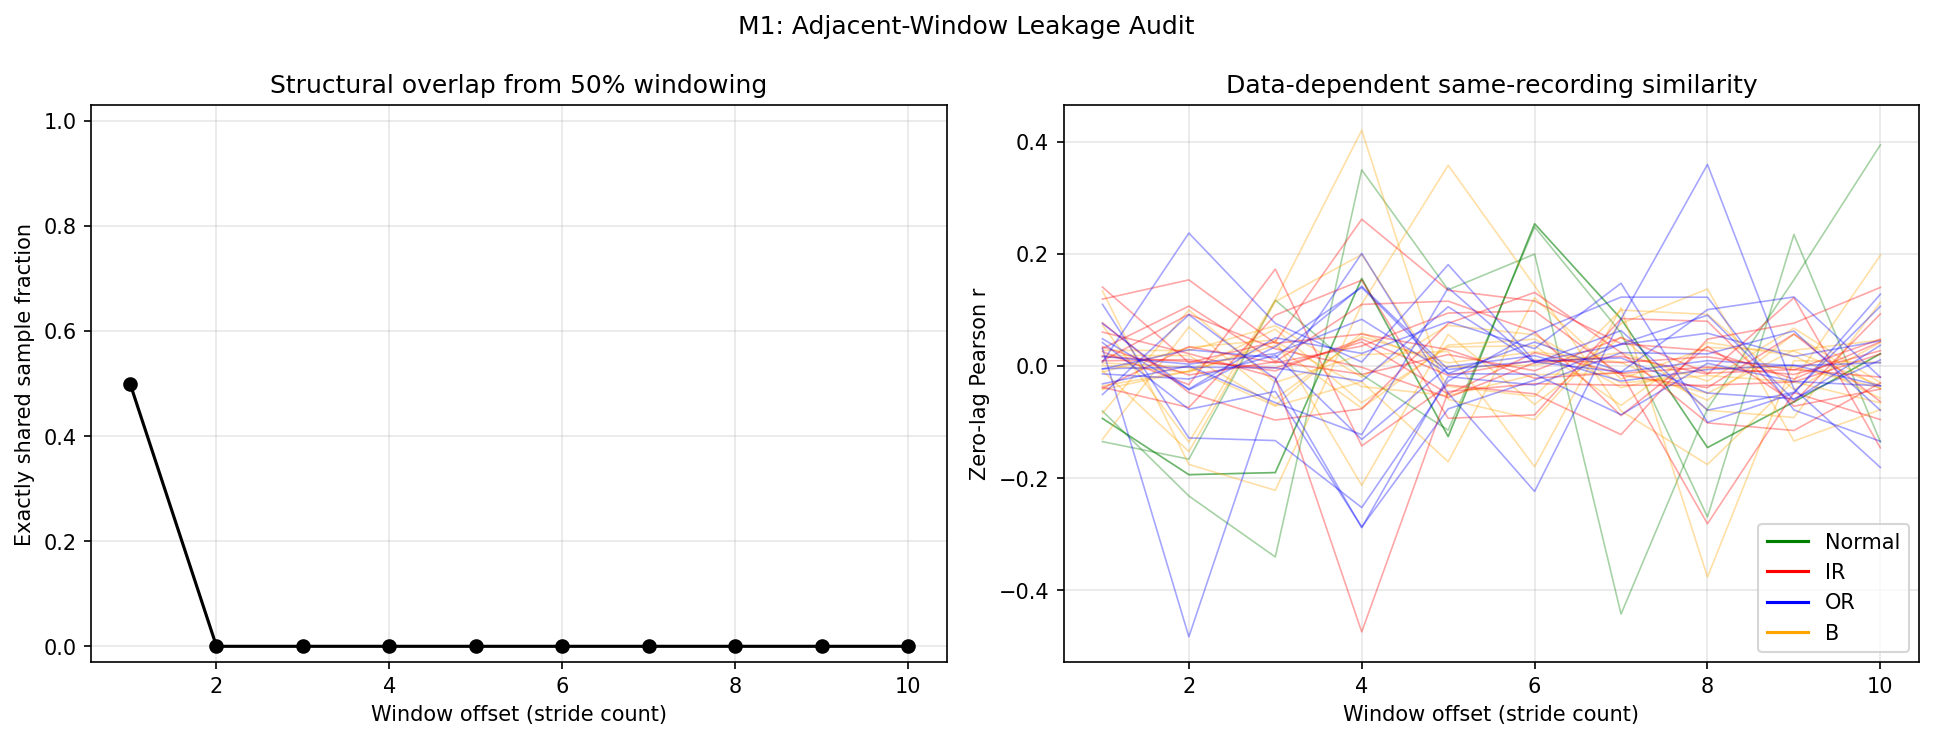
\includegraphics[width=\textwidth]{../results/figures/m1_adjacent_autocorrelation.png}
\caption{M1: Structural adjacent-window overlap and data-dependent zero-lag similarity.}
\label{fig:m1}
\end{figure}

\subsection{Fault-Band Energy Audit (M5)}

% [M5故障频带能量审计]：对称保真度同时惩罚放大与衰减；该单一指标不等同于完整物理安全性。
For each augmentation, we compute a symmetric energy-fidelity score
\[
F_{\text{energy}}=
\min\left(
\frac{E_{\text{aug}}}{E_{\text{orig}}},
\frac{E_{\text{orig}}}{E_{\text{aug}}}
\right)
\]
in envelope-spectrum neighborhoods around the first three harmonics of the relevant bearing frequency (BPFO, BPFI, or BSF). The score lies in $[0,1]$ and penalizes attenuation and amplification equally, avoiding the error of treating broadband energy injection as preservation.

\begin{figure}[H]
\centering
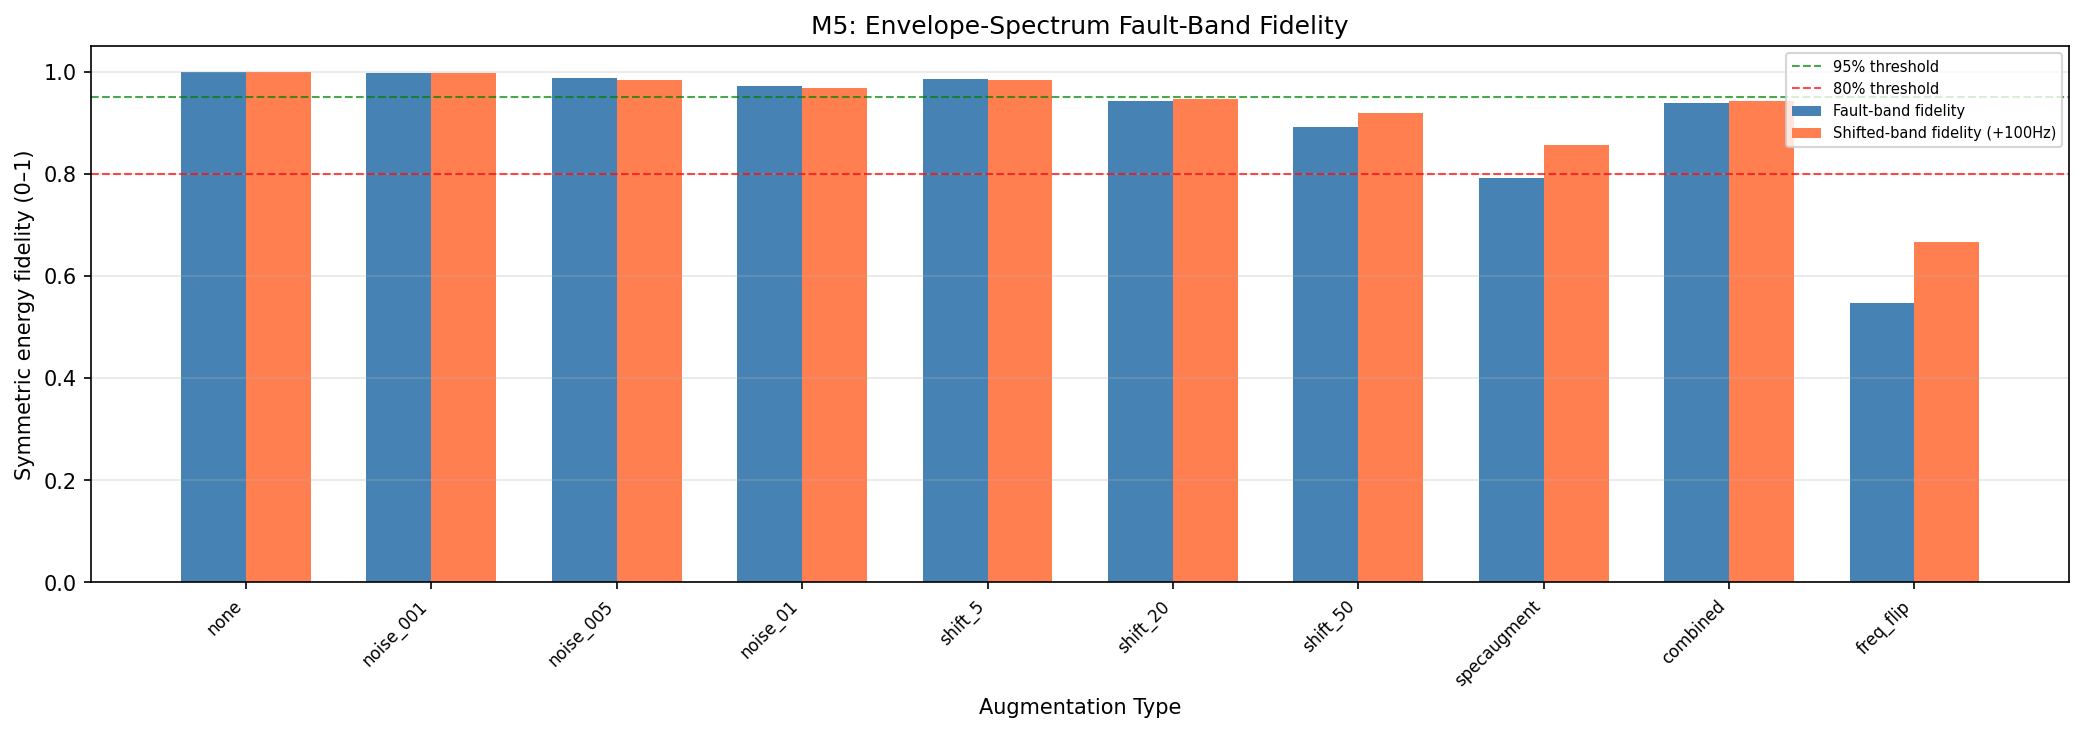
\includegraphics[width=\textwidth]{../results/figures/m5_fault_band_energy.png}
\caption{M5: Symmetric envelope-spectrum fault-band energy fidelity ($F_{\text{energy}}$).}
\label{fig:m5}
\end{figure}

\subsection{Feature Diversity Analysis (M2)}

% [M2输入表示多样性]：使用确定性 STFT 输入距离，不赋予未训练网络隐藏层以语义。
For 200 paired training samples, we compute standardized $32\times32$ STFT magnitude representations before and after augmentation, then measure paired cosine distance and SVD effective rank (Figure~\ref{fig:m2}). This deterministic input-representation audit avoids attributing meaning to an untrained network's hidden layer.

\begin{figure}[H]
\centering
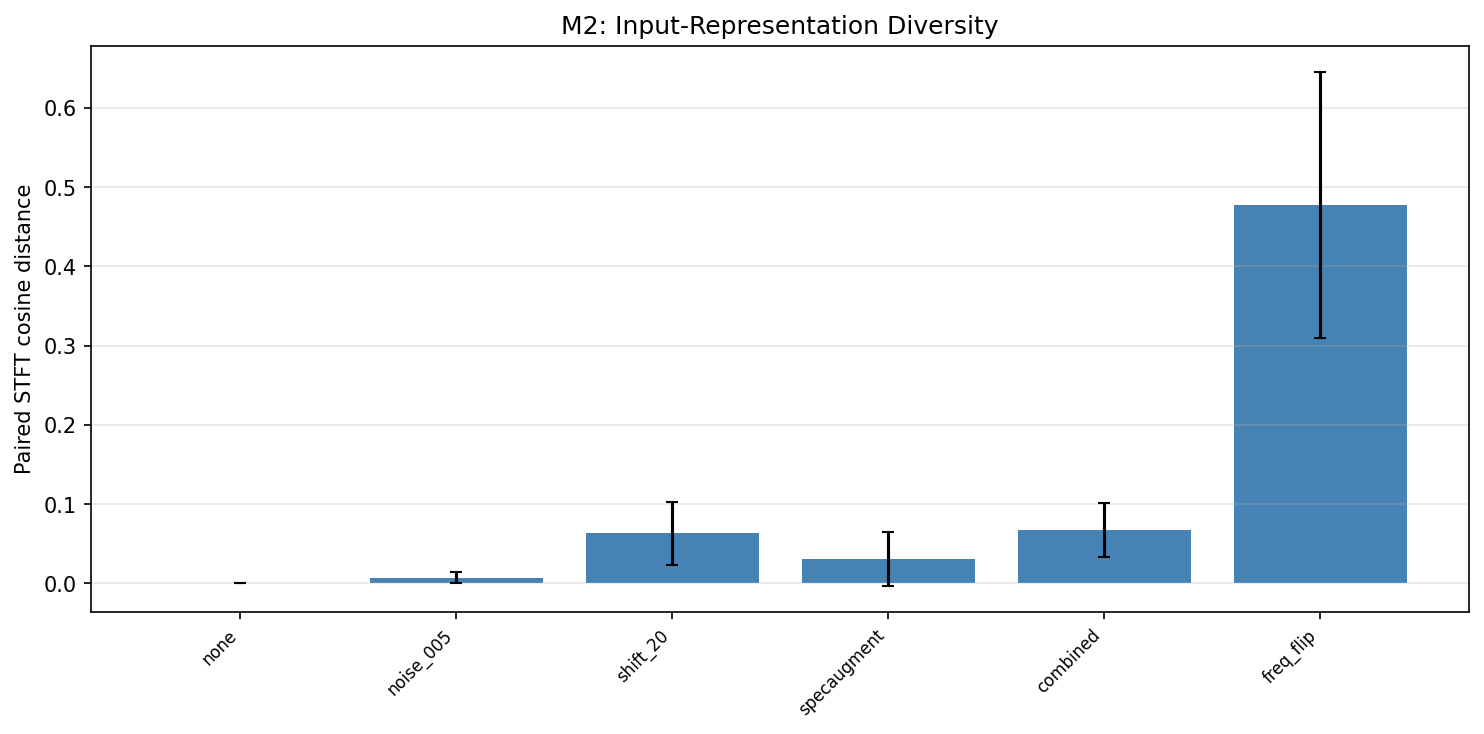
\includegraphics[width=0.7\textwidth]{../results/figures/m2_feature_diversity.png}
\caption{M2: Input-representation diversity (paired STFT cosine distance).}
\label{fig:m2}
\end{figure}

\begin{figure}[H]
\centering
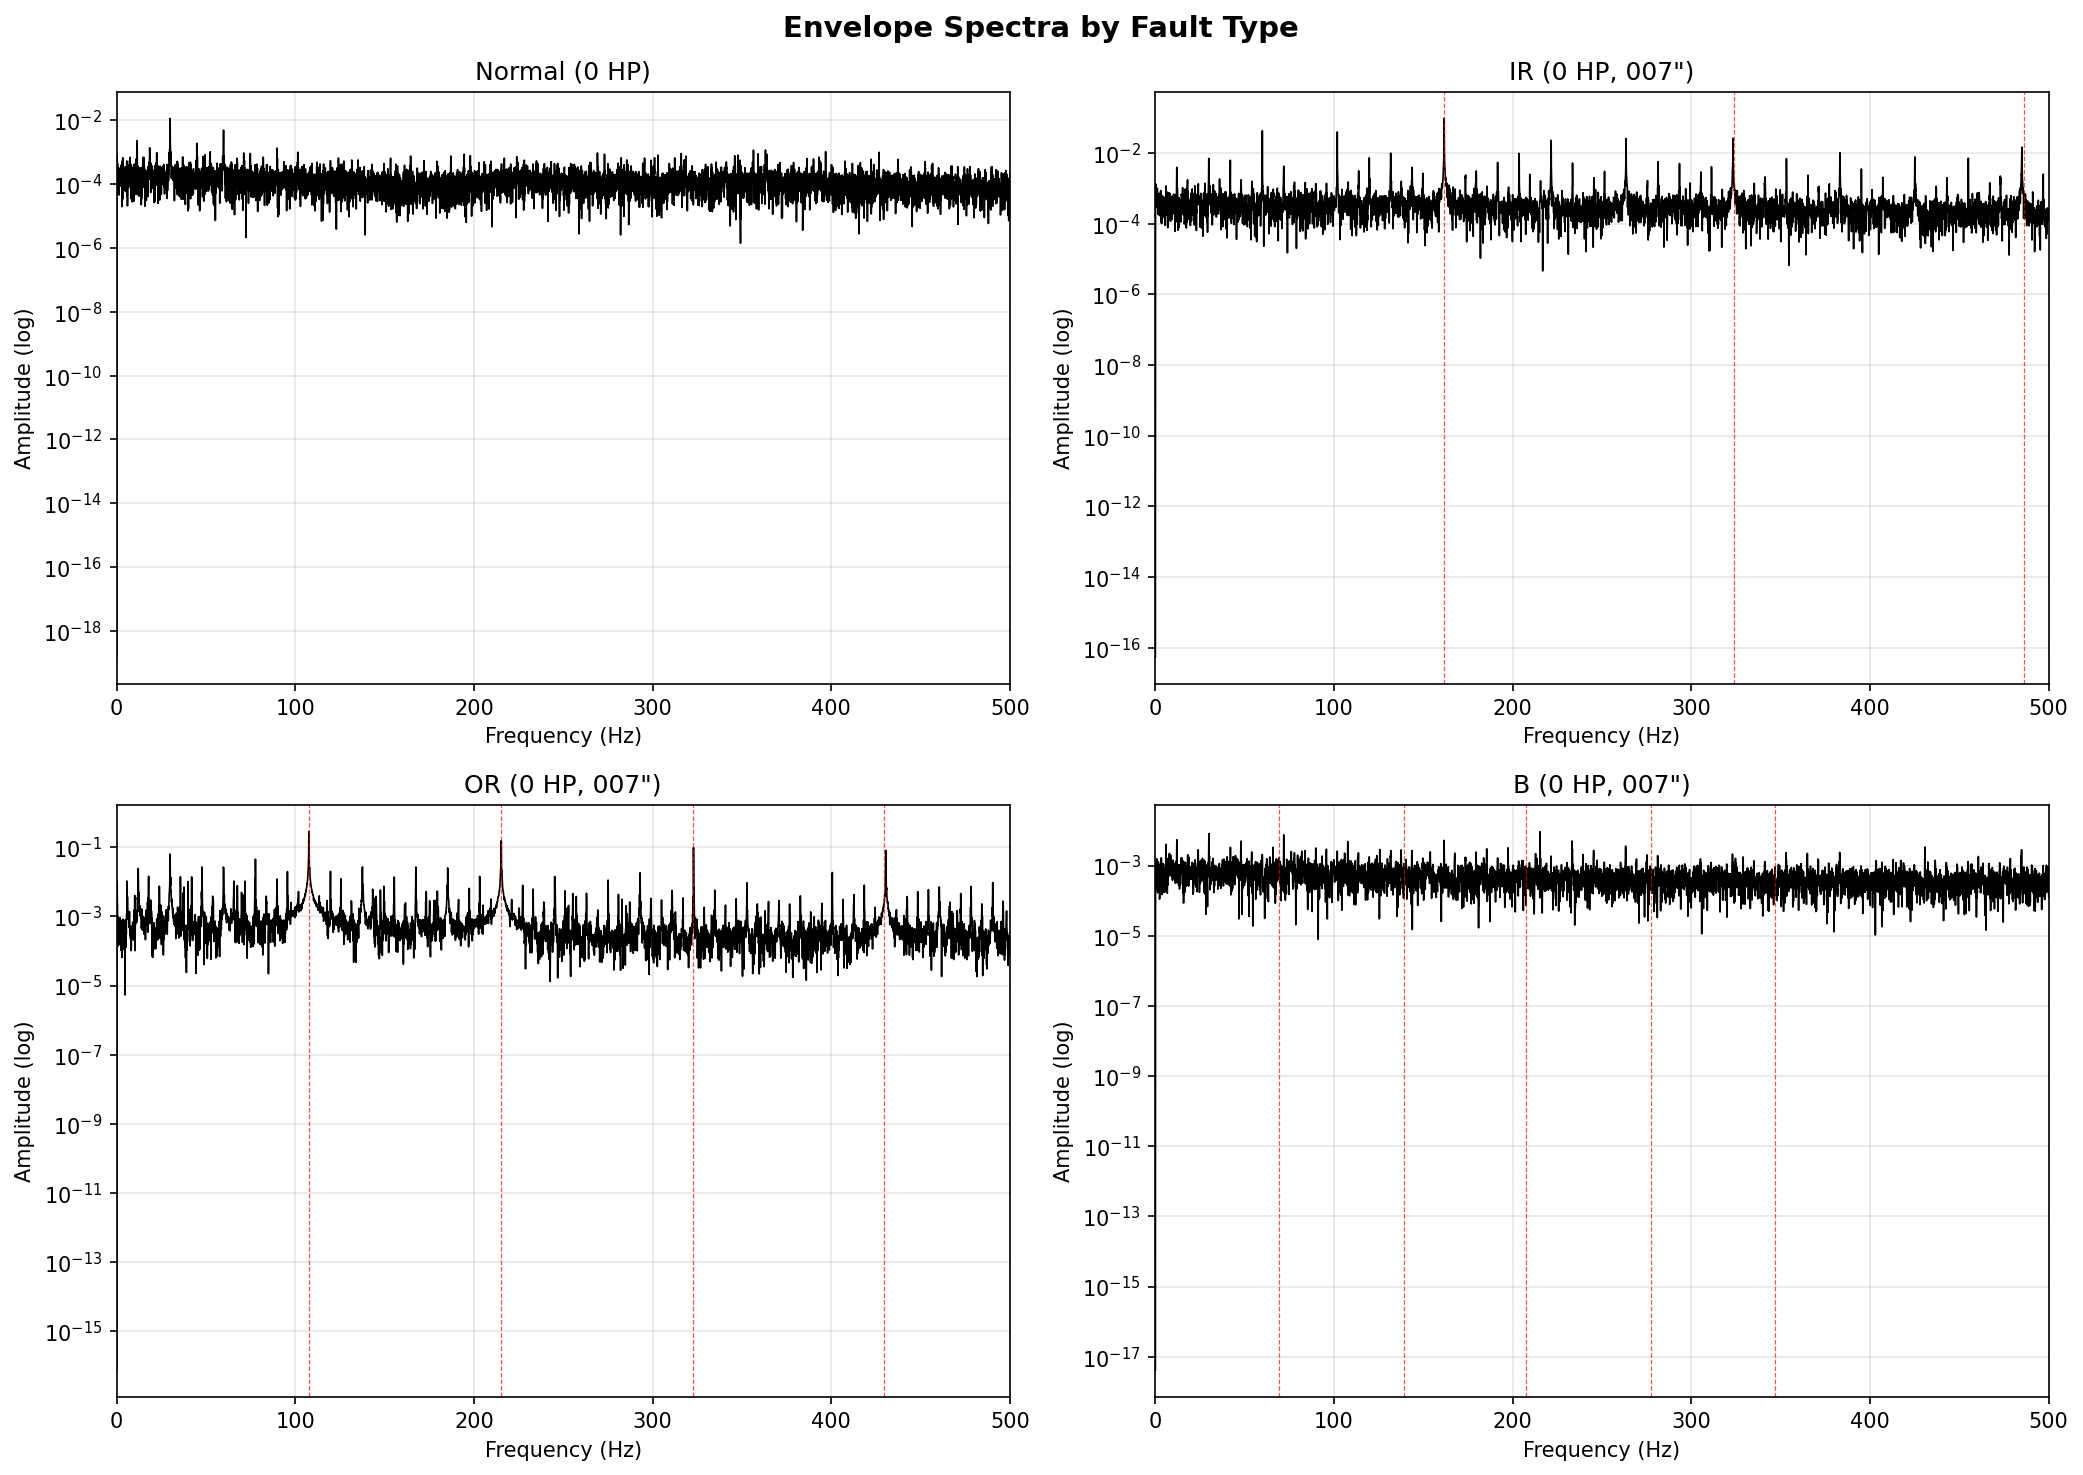
\includegraphics[width=\textwidth]{../results/figures/envelope_spectra_examples.png}
\caption{Envelope spectrum examples for each fault class.}
\label{fig:env}
\end{figure}

% ================================================================
\section{Experimental Setup}
% ================================================================

% [实验设置]：最佳验证 epoch 仅作为审计诊断，不能证明形式收敛。
\begin{itemize}[nosep]
    \item \textbf{Hardware}: Baidu Cloud BCC, NVIDIA A10 (24\,GB), Ubuntu 22.04;\newline PyTorch 2.5.1+cu121
    \item \textbf{Training}: Adam ($\text{lr}=0.001$), CrossEntropy loss, batch\_size=128, 50 epochs
    \item \textbf{Normalization}: Z-score computed on training set only
    \item \textbf{Metrics}: Accuracy, macro-F1, per-class precision/recall/F1
    \item \textbf{Statistics}: Mean $\pm$ std across 5 seeds; Cohen's $d$ for effect size
    \item \textbf{Best-validation epoch diagnostic}: mean 12.58, median 7, maximum 50; 8/200 runs attain their best validation accuracy in epochs 45--50 (Figure~\ref{fig:convergence}).
\end{itemize}

\begin{figure}[H]
\centering
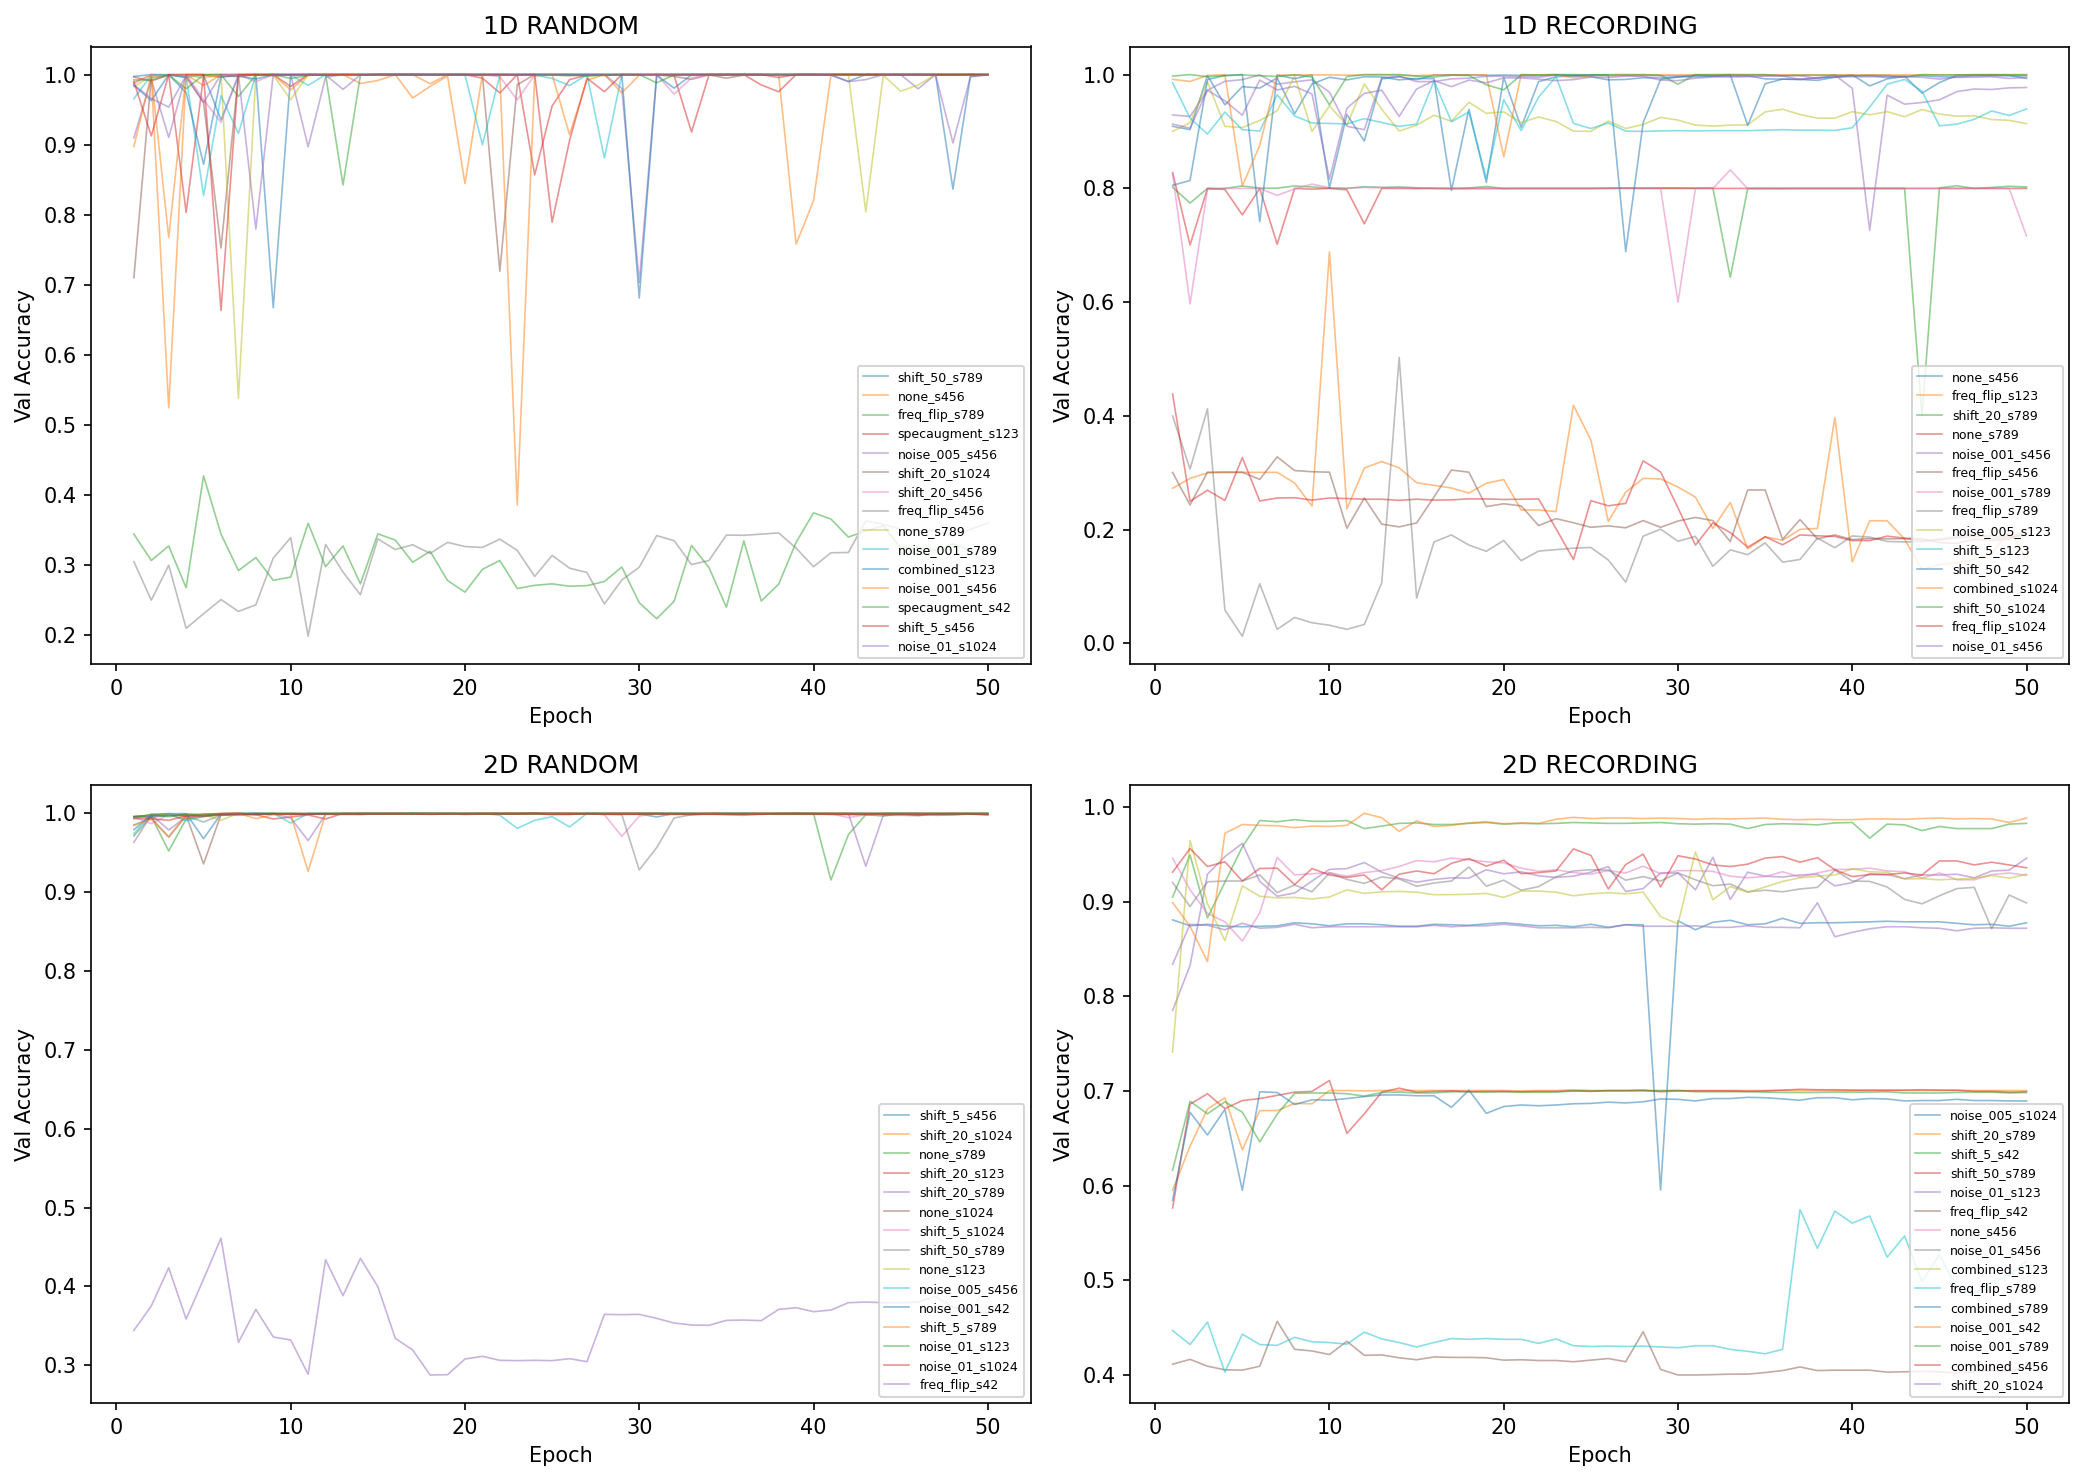
\includegraphics[width=\textwidth]{../results/figures/convergence_curves.png}
\caption{Convergence curves for all 200 training runs across four configurations.}
\label{fig:convergence}
\end{figure}

% ================================================================
\section{Results}
\label{sec:results}
% ================================================================

\subsection{Main Factorial Results}

% [Table 1解读]：写论文最怕的就是表格数据没人读，所以一定要在正文里解读关键数字。这里挑出gap和d值，引导审稿人关注最重要的发现。
Table~\ref{tab:main} reports all 40 configurations. The no-augmentation random-window baselines are 0.9998 (1D) and 0.9999 (2D), compared with 0.9429 and 0.8856 under recording-level splitting. The corresponding protocol gaps are 0.0569 and 0.1143; pooled-SD Cohen's $d$ is 0.9262 and 1.4697 (Figure~\ref{fig:cohens}). The physically plausible random-split augmentations remain near ceiling, whereas the destructive negative control drops to 0.4069 and 0.4488.

\begin{figure}[H]
\centering
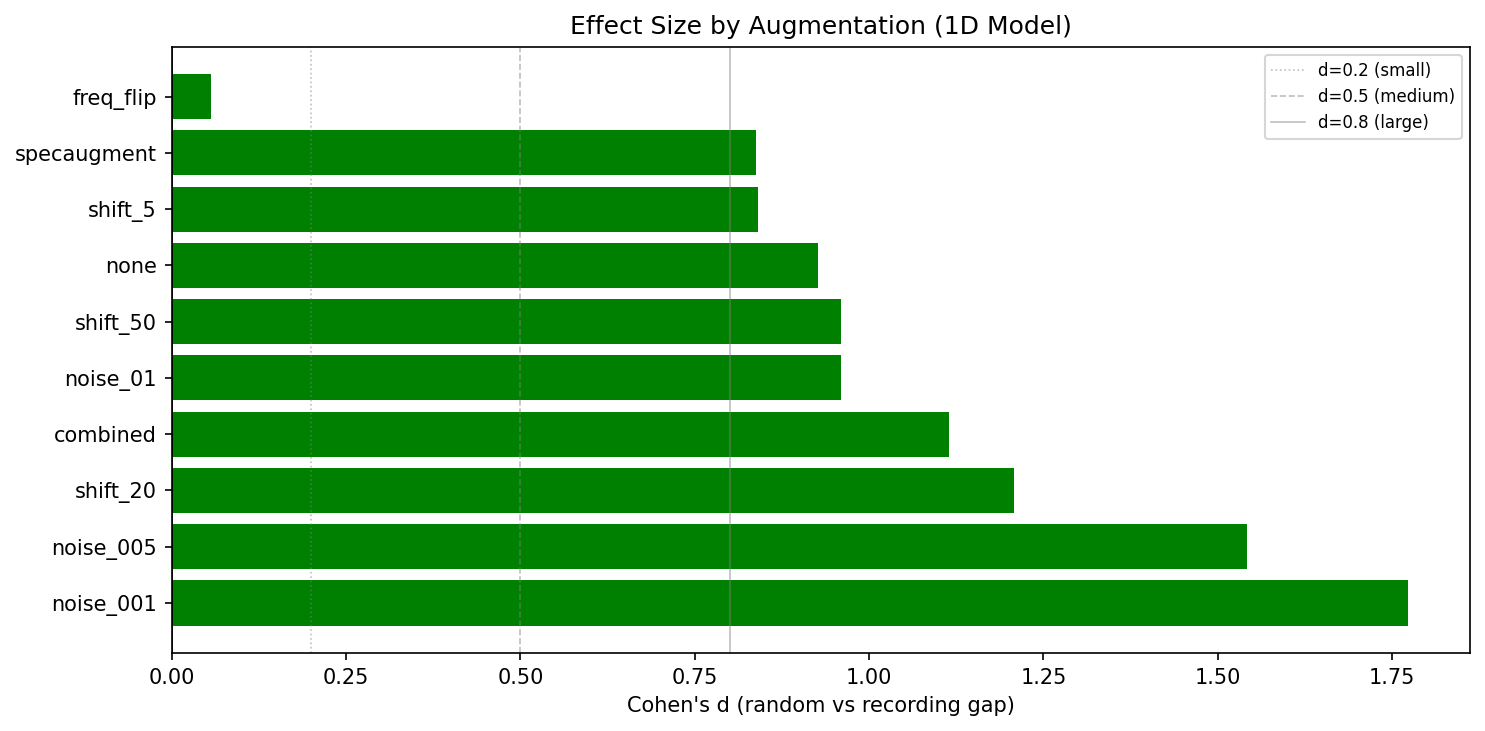
\includegraphics[width=0.48\textwidth]{../results/figures/cohens_d_1d.png}
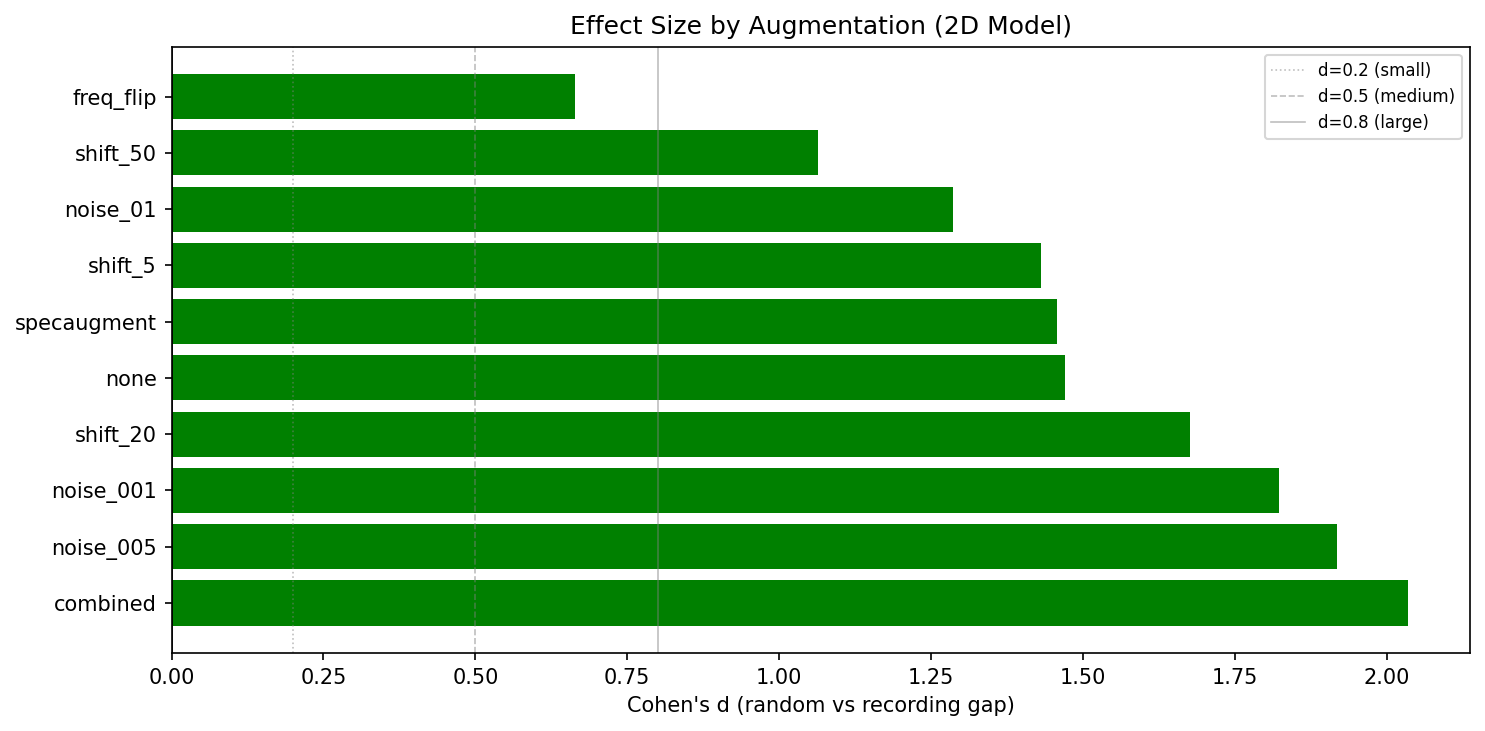
\includegraphics[width=0.48\textwidth]{../results/figures/cohens_d_2d.png}
\caption{Cohen's $d$ effect sizes. Left: 1D-CNN. Right: 2D-CNN.}
\label{fig:cohens}
\end{figure}

% AUTO-GENERATED by src/summarize_results.py; do not hand-edit.
\begin{table}[htbp]
\centering
\caption{Main results: accuracy (mean $\pm$ std) across 5 seeds.}
\label{tab:main}
\resizebox{\textwidth}{!}{%
\begin{tabular}{lcccc}
\toprule
Augmentation & 1D Random & 1D Recording & 2D Random & 2D Recording \\
\midrule
None & 0.9998 $\pm$ 0.0002 & 0.9429 $\pm$ 0.0777 & 0.9999 $\pm$ 0.0002 & 0.8856 $\pm$ 0.0984 \\
Noise 0.01 & 0.9999 $\pm$ 0.0002 & 0.9379 $\pm$ 0.0443 & 0.9997 $\pm$ 0.0003 & 0.8807 $\pm$ 0.0826 \\
Noise 0.05 & 0.9999 $\pm$ 0.0002 & 0.9628 $\pm$ 0.0305 & 0.9998 $\pm$ 0.0002 & 0.8900 $\pm$ 0.0724 \\
Noise 0.10 & 0.9997 $\pm$ 0.0005 & 0.9351 $\pm$ 0.0851 & 0.9997 $\pm$ 0.0003 & 0.9188 $\pm$ 0.0795 \\
Shift 5 & 0.9999 $\pm$ 0.0002 & 0.9728 $\pm$ 0.0407 & 0.9997 $\pm$ 0.0005 & 0.9229 $\pm$ 0.0679 \\
Shift 20 & 0.9997 $\pm$ 0.0004 & 0.9267 $\pm$ 0.0764 & 0.9997 $\pm$ 0.0003 & 0.9091 $\pm$ 0.0683 \\
Shift 50 & 0.9999 $\pm$ 0.0002 & 0.9396 $\pm$ 0.0795 & 0.9997 $\pm$ 0.0005 & 0.8477 $\pm$ 0.1808 \\
Spectral/time mask & 0.9999 $\pm$ 0.0002 & 0.9439 $\pm$ 0.0845 & 0.9995 $\pm$ 0.0005 & 0.9009 $\pm$ 0.0856 \\
Combined & 0.9999 $\pm$ 0.0002 & 0.9334 $\pm$ 0.0755 & 0.9997 $\pm$ 0.0005 & 0.8960 $\pm$ 0.0645 \\
FFT magnitude reversal & 0.4069 $\pm$ 0.0377 & 0.4026 $\pm$ 0.0882 & 0.4488 $\pm$ 0.0369 & 0.3919 $\pm$ 0.1019 \\
\bottomrule
\end{tabular}
}
\end{table}


Table~\ref{tab:macro-f1} reports the required Macro-F1 results for all 40 configurations. Under recording-level splitting, Macro-F1 changes from 0.9365 to 0.9699 for 1D and from 0.8717 to 0.9187 for 2D when the 5-sample shift is applied; the destructive control falls to 0.3337 and 0.2911.

% AUTO-GENERATED by src/summarize_results.py; do not hand-edit.
\begin{table}[htbp]
\centering
\caption{Macro-F1 (mean $\pm$ std) across 5 seeds for all factorial configurations.}
\label{tab:macro-f1}
\resizebox{\textwidth}{!}{%
\begin{tabular}{lcccc}
\toprule
Augmentation & 1D Random & 1D Recording & 2D Random & 2D Recording \\
\midrule
None & 0.9998 $\pm$ 0.0002 & 0.9365 $\pm$ 0.0872 & 0.9999 $\pm$ 0.0002 & 0.8717 $\pm$ 0.1146 \\
Noise 0.01 & 0.9999 $\pm$ 0.0002 & 0.9393 $\pm$ 0.0410 & 0.9997 $\pm$ 0.0003 & 0.8771 $\pm$ 0.0804 \\
Noise 0.05 & 0.9999 $\pm$ 0.0002 & 0.9618 $\pm$ 0.0342 & 0.9998 $\pm$ 0.0002 & 0.8868 $\pm$ 0.0724 \\
Noise 0.10 & 0.9997 $\pm$ 0.0005 & 0.9173 $\pm$ 0.1217 & 0.9997 $\pm$ 0.0003 & 0.9145 $\pm$ 0.0801 \\
Shift 5 & 0.9999 $\pm$ 0.0002 & 0.9699 $\pm$ 0.0473 & 0.9997 $\pm$ 0.0005 & 0.9187 $\pm$ 0.0700 \\
Shift 20 & 0.9996 $\pm$ 0.0004 & 0.9159 $\pm$ 0.0964 & 0.9997 $\pm$ 0.0003 & 0.9055 $\pm$ 0.0689 \\
Shift 50 & 0.9999 $\pm$ 0.0002 & 0.9430 $\pm$ 0.0712 & 0.9997 $\pm$ 0.0005 & 0.8337 $\pm$ 0.2010 \\
Spectral/time mask & 0.9999 $\pm$ 0.0002 & 0.9247 $\pm$ 0.1239 & 0.9995 $\pm$ 0.0005 & 0.8946 $\pm$ 0.0889 \\
Combined & 0.9999 $\pm$ 0.0002 & 0.9193 $\pm$ 0.1059 & 0.9997 $\pm$ 0.0005 & 0.8951 $\pm$ 0.0599 \\
FFT magnitude reversal & 0.3527 $\pm$ 0.0526 & 0.3337 $\pm$ 0.1076 & 0.3414 $\pm$ 0.0460 & 0.2911 $\pm$ 0.0977 \\
\bottomrule
\end{tabular}
}
\end{table}


% [模型依赖结果]：明确报告每个模型中高于和低于无增强均值的条件，并保留负对照。
For 1D-CNN under recording-level splitting, three of nine augmentations improve on the 0.9429 baseline; for 2D-CNN, six improve on the 0.8856 baseline. A 5-sample shift is best for both models (0.9728 and 0.9229). The frequency-reversal negative control performs worst (0.4026 and 0.3919), supporting its role as a destructive check. Figures~\ref{fig:rvr1d}--\ref{fig:rvr2d} visualize the contrast.

\begin{figure}[H]
\centering
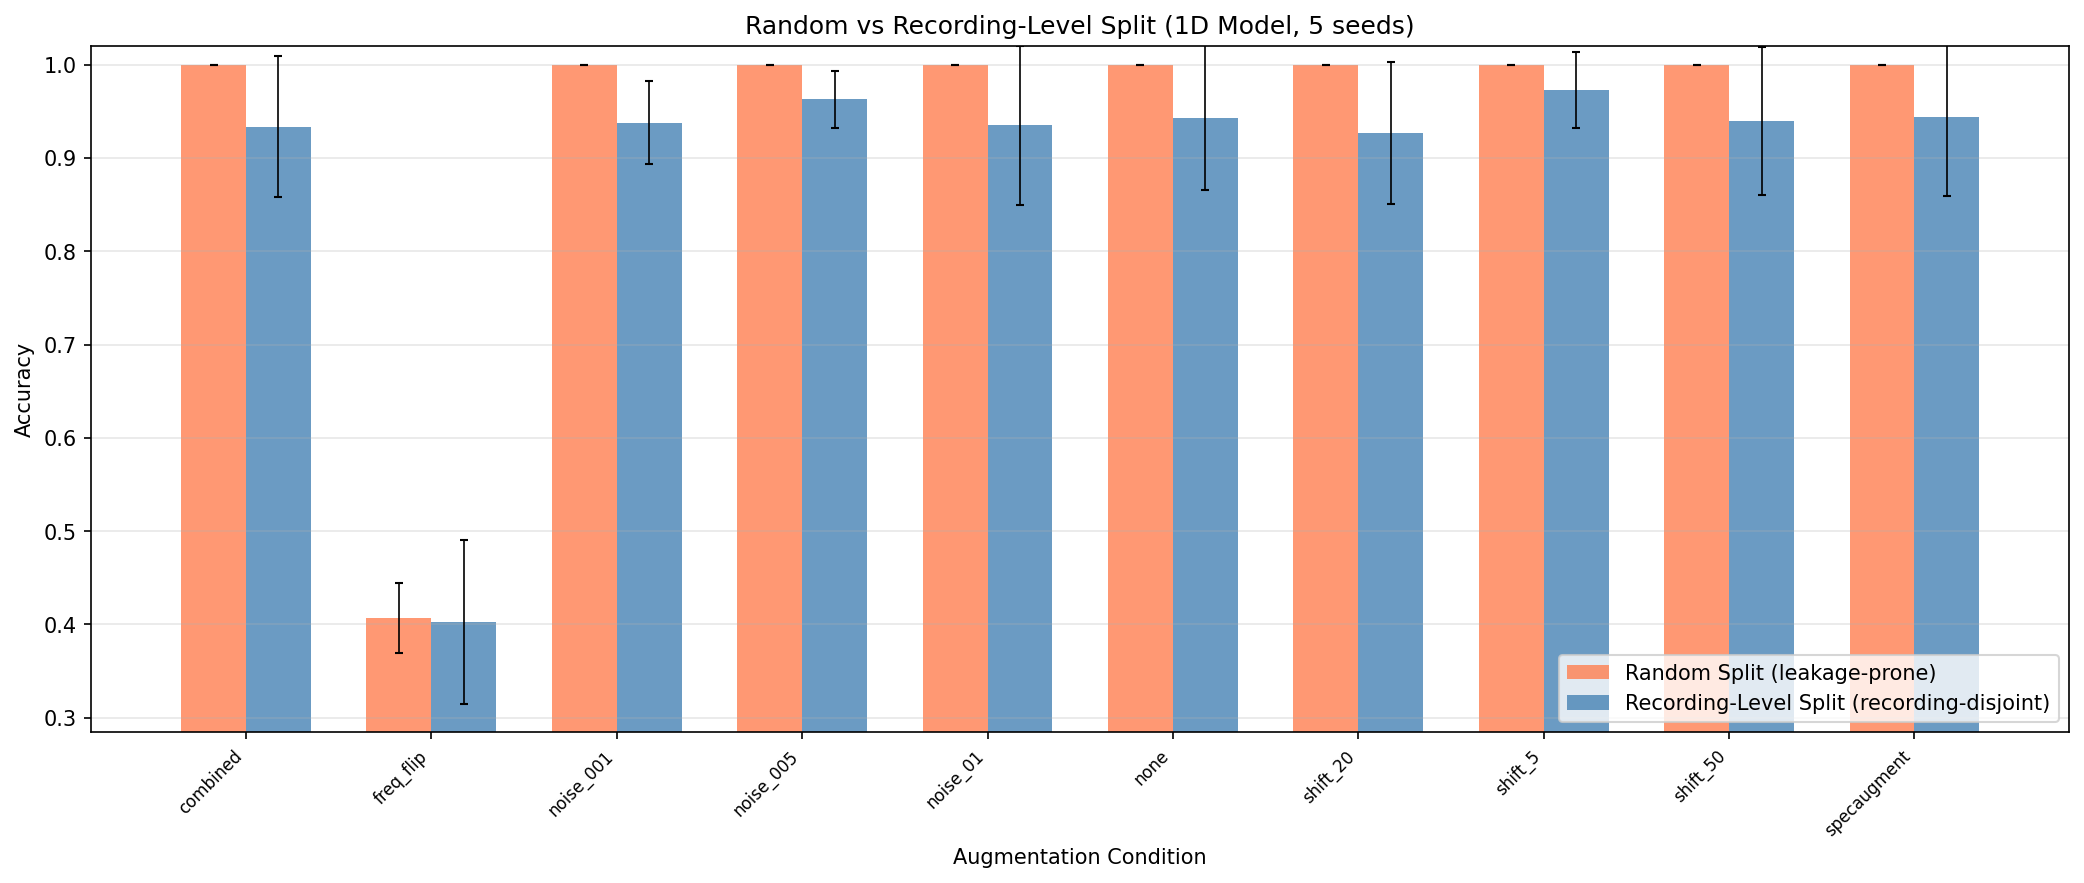
\includegraphics[width=\textwidth]{../results/figures/random_vs_recording_1d.png}
\caption{Random vs.\ recording-level split accuracy (1D-CNN).}
\label{fig:rvr1d}
\end{figure}

\begin{figure}[H]
\centering
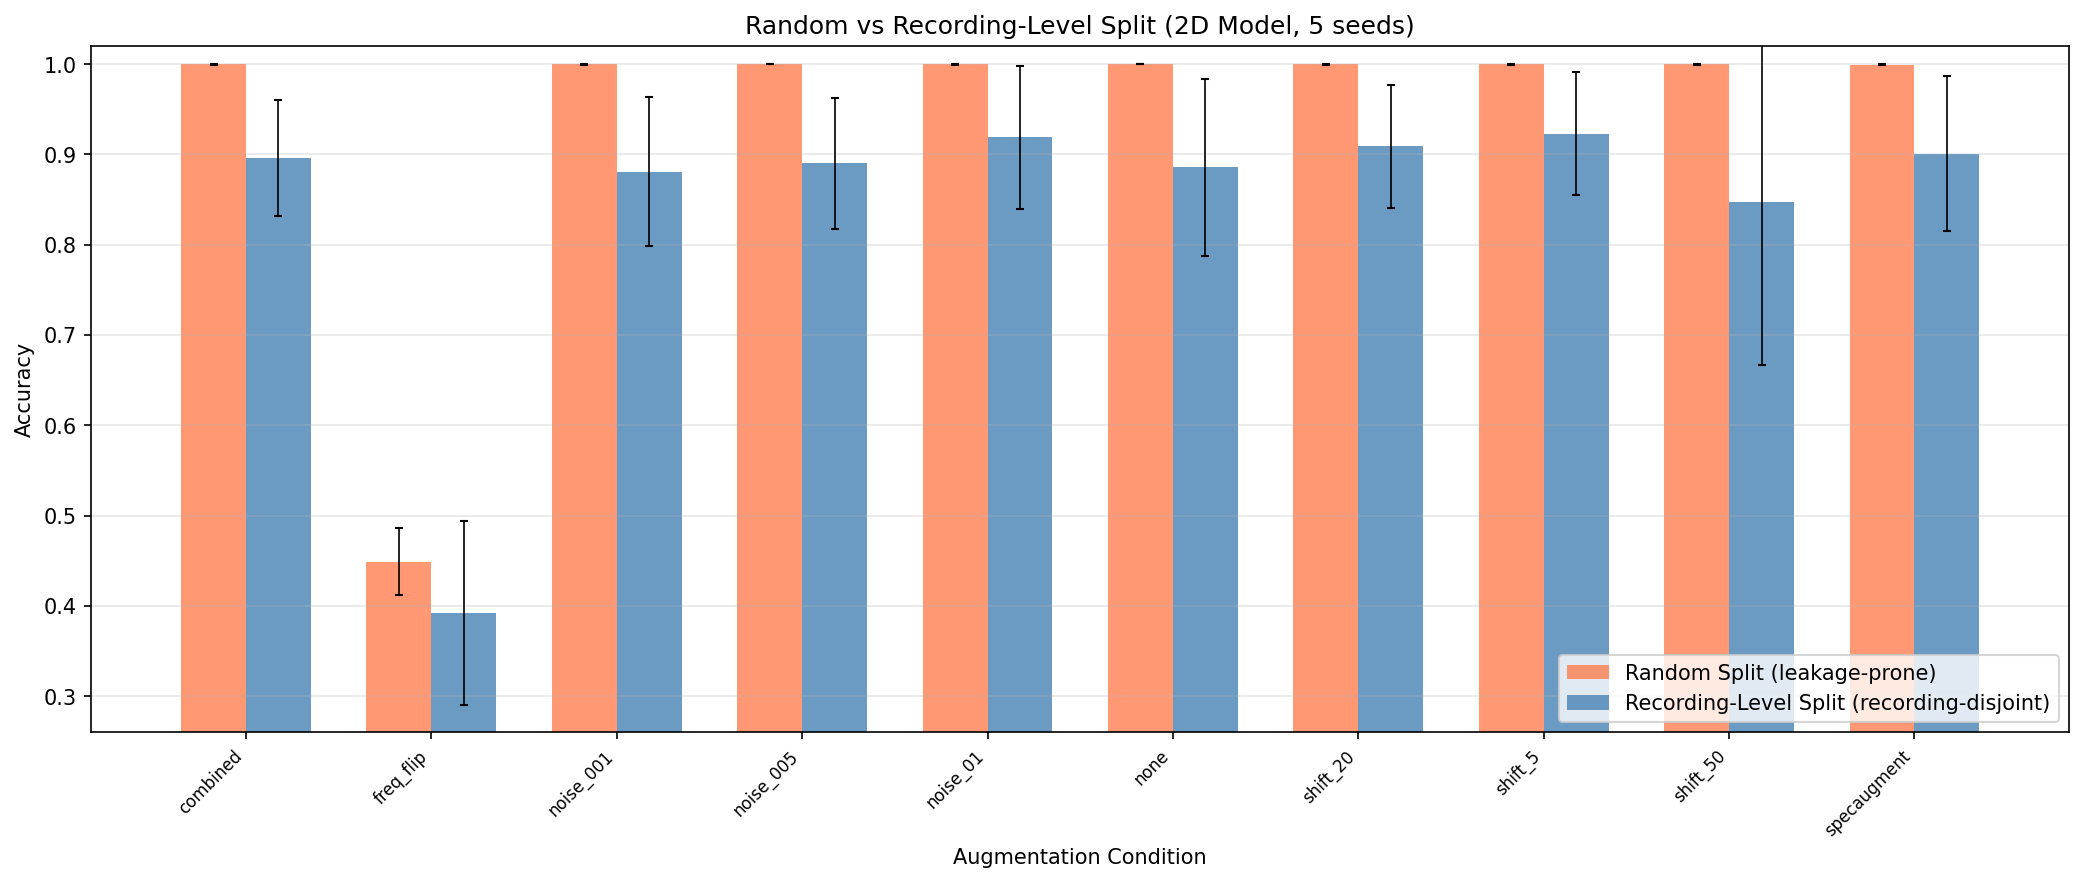
\includegraphics[width=\textwidth]{../results/figures/random_vs_recording_2d.png}
\caption{Random vs.\ recording-level split accuracy (2D-CNN).}
\label{fig:rvr2d}
\end{figure}

\subsection{Per-Class Analysis}

% [Per-class结果解读]：不要避免指出最差类（IR和B）。诚实报告每个类的短板比只报平均指标更有说服力。
Table~\ref{tab:perclass} reports 2D-CNN recording-level per-class F1. Excluding the deliberately destructive negative control, Normal is 0.9996--1.0000, while IR, OR, and Ball span 0.742--0.861, 0.730--0.892, and 0.753--0.943. Under frequency reversal, IR F1 falls to zero and the other classes also deteriorate sharply.

% AUTO-GENERATED by src/summarize_results.py; do not hand-edit.
\begin{table}[htbp]
\centering
\caption{Per-class F1 under recording-level splitting for the 2D-CNN (mean $\pm$ std).}
\label{tab:perclass}
\begin{tabular}{lcccc}
\toprule
Augmentation & Normal & IR & OR & Ball \\
\midrule
None & 1.000 $\pm$ 0.000 & 0.742 $\pm$ 0.293 & 0.838 $\pm$ 0.137 & 0.906 $\pm$ 0.057 \\
Noise 0.01 & 1.000 $\pm$ 0.000 & 0.817 $\pm$ 0.199 & 0.827 $\pm$ 0.111 & 0.864 $\pm$ 0.091 \\
Noise 0.05 & 1.000 $\pm$ 0.000 & 0.803 $\pm$ 0.192 & 0.858 $\pm$ 0.116 & 0.886 $\pm$ 0.076 \\
Noise 0.10 & 1.000 $\pm$ 0.000 & 0.843 $\pm$ 0.202 & 0.891 $\pm$ 0.117 & 0.924 $\pm$ 0.061 \\
Shift 5 & 1.000 $\pm$ 0.001 & 0.848 $\pm$ 0.184 & 0.884 $\pm$ 0.104 & 0.943 $\pm$ 0.069 \\
Shift 20 & 1.000 $\pm$ 0.000 & 0.831 $\pm$ 0.190 & 0.877 $\pm$ 0.099 & 0.914 $\pm$ 0.053 \\
Shift 50 & 1.000 $\pm$ 0.000 & 0.851 $\pm$ 0.172 & 0.730 $\pm$ 0.371 & 0.753 $\pm$ 0.286 \\
Spectral/time mask & 1.000 $\pm$ 0.000 & 0.802 $\pm$ 0.230 & 0.859 $\pm$ 0.112 & 0.918 $\pm$ 0.052 \\
Combined & 1.000 $\pm$ 0.000 & 0.861 $\pm$ 0.109 & 0.850 $\pm$ 0.118 & 0.870 $\pm$ 0.079 \\
FFT magnitude reversal & 0.568 $\pm$ 0.205 & 0.000 $\pm$ 0.000 & 0.453 $\pm$ 0.272 & 0.144 $\pm$ 0.132 \\
\bottomrule
\end{tabular}
\end{table}


Table~\ref{tab:perclass-prf} adds per-class precision and recall for both models under the no-augmentation baseline, the best augmentation, and the destructive control. This prevents the aggregate metrics from hiding asymmetric class failures; in particular, the negative control drives 2D-CNN IR recall to zero.

% AUTO-GENERATED by src/summarize_results.py; do not hand-edit.
\begin{table}[htbp]
\centering
\caption{Recording-level per-class precision, recall, and F1 (mean $\pm$ std across 5 seeds) for the baseline, best augmentation, and destructive control.}
\label{tab:perclass-prf}
\resizebox{\textwidth}{!}{%
\begin{tabular}{lllcccc}
\toprule
Model & Augmentation & Metric & Normal & IR & OR & Ball \\
\midrule
CNN--1D & None & Precision & 0.997 $\pm$ 0.007 & 0.947 $\pm$ 0.096 & 0.934 $\pm$ 0.116 & 0.958 $\pm$ 0.085 \\
 &  & Recall & 1.000 $\pm$ 0.000 & 0.939 $\pm$ 0.121 & 1.000 $\pm$ 0.000 & 0.841 $\pm$ 0.294 \\
 &  & F1 & 0.998 $\pm$ 0.003 & 0.934 $\pm$ 0.077 & 0.962 $\pm$ 0.068 & 0.852 $\pm$ 0.229 \\
\addlinespace
 & Shift 5 & Precision & 0.994 $\pm$ 0.012 & 0.987 $\pm$ 0.016 & 0.998 $\pm$ 0.004 & 0.937 $\pm$ 0.125 \\
 &  & Recall & 1.000 $\pm$ 0.000 & 0.906 $\pm$ 0.187 & 1.000 $\pm$ 0.000 & 0.978 $\pm$ 0.022 \\
 &  & F1 & 0.997 $\pm$ 0.006 & 0.932 $\pm$ 0.119 & 0.999 $\pm$ 0.002 & 0.952 $\pm$ 0.070 \\
\addlinespace
 & FFT magnitude reversal & Precision & 0.522 $\pm$ 0.443 & 0.226 $\pm$ 0.169 & 0.275 $\pm$ 0.075 & 0.788 $\pm$ 0.395 \\
 &  & Recall & 0.600 $\pm$ 0.490 & 0.336 $\pm$ 0.322 & 0.512 $\pm$ 0.319 & 0.124 $\pm$ 0.117 \\
 &  & F1 & 0.554 $\pm$ 0.458 & 0.253 $\pm$ 0.214 & 0.325 $\pm$ 0.144 & 0.202 $\pm$ 0.183 \\
\addlinespace
\midrule
CNN--2D & None & Precision & 1.000 $\pm$ 0.000 & 0.940 $\pm$ 0.078 & 0.822 $\pm$ 0.196 & 0.868 $\pm$ 0.111 \\
 &  & Recall & 1.000 $\pm$ 0.000 & 0.696 $\pm$ 0.360 & 0.884 $\pm$ 0.113 & 0.960 $\pm$ 0.041 \\
 &  & F1 & 1.000 $\pm$ 0.000 & 0.742 $\pm$ 0.293 & 0.838 $\pm$ 0.137 & 0.906 $\pm$ 0.057 \\
\addlinespace
 & Shift 5 & Precision & 1.000 $\pm$ 0.000 & 0.969 $\pm$ 0.031 & 0.879 $\pm$ 0.163 & 0.925 $\pm$ 0.101 \\
 &  & Recall & 0.999 $\pm$ 0.002 & 0.803 $\pm$ 0.260 & 0.926 $\pm$ 0.130 & 0.965 $\pm$ 0.035 \\
 &  & F1 & 1.000 $\pm$ 0.001 & 0.848 $\pm$ 0.184 & 0.884 $\pm$ 0.104 & 0.943 $\pm$ 0.069 \\
\addlinespace
 & FFT magnitude reversal & Precision & 0.438 $\pm$ 0.168 & 0.000 $\pm$ 0.000 & 0.367 $\pm$ 0.244 & 0.354 $\pm$ 0.135 \\
 &  & Recall & 0.843 $\pm$ 0.301 & 0.000 $\pm$ 0.000 & 0.624 $\pm$ 0.339 & 0.120 $\pm$ 0.119 \\
 &  & F1 & 0.568 $\pm$ 0.205 & 0.000 $\pm$ 0.000 & 0.453 $\pm$ 0.272 & 0.144 $\pm$ 0.132 \\
\bottomrule
\end{tabular}
}
\end{table}


Per-class heatmaps for both models are provided in Figure~\ref{fig:pc}.

\begin{figure}[H]
\centering
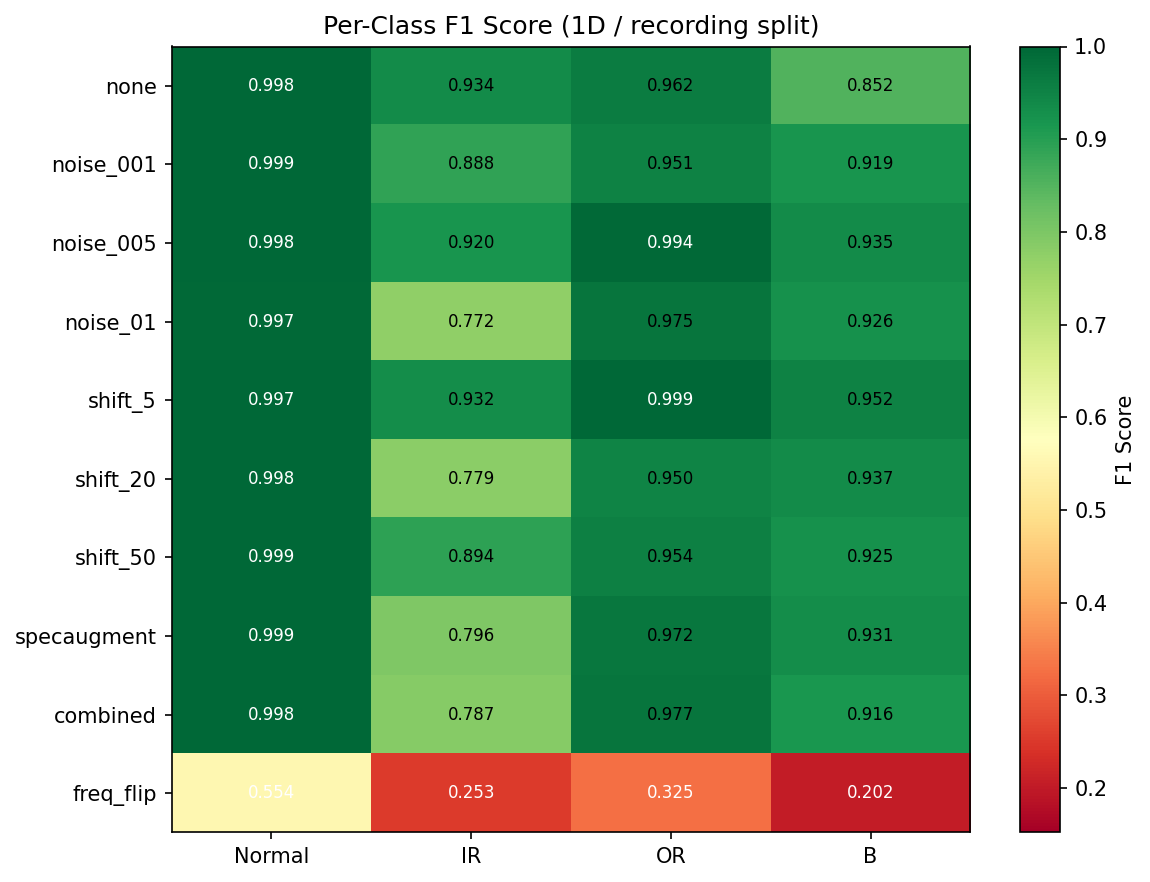
\includegraphics[width=0.48\textwidth]{../results/figures/per_class_1d_recording.png}
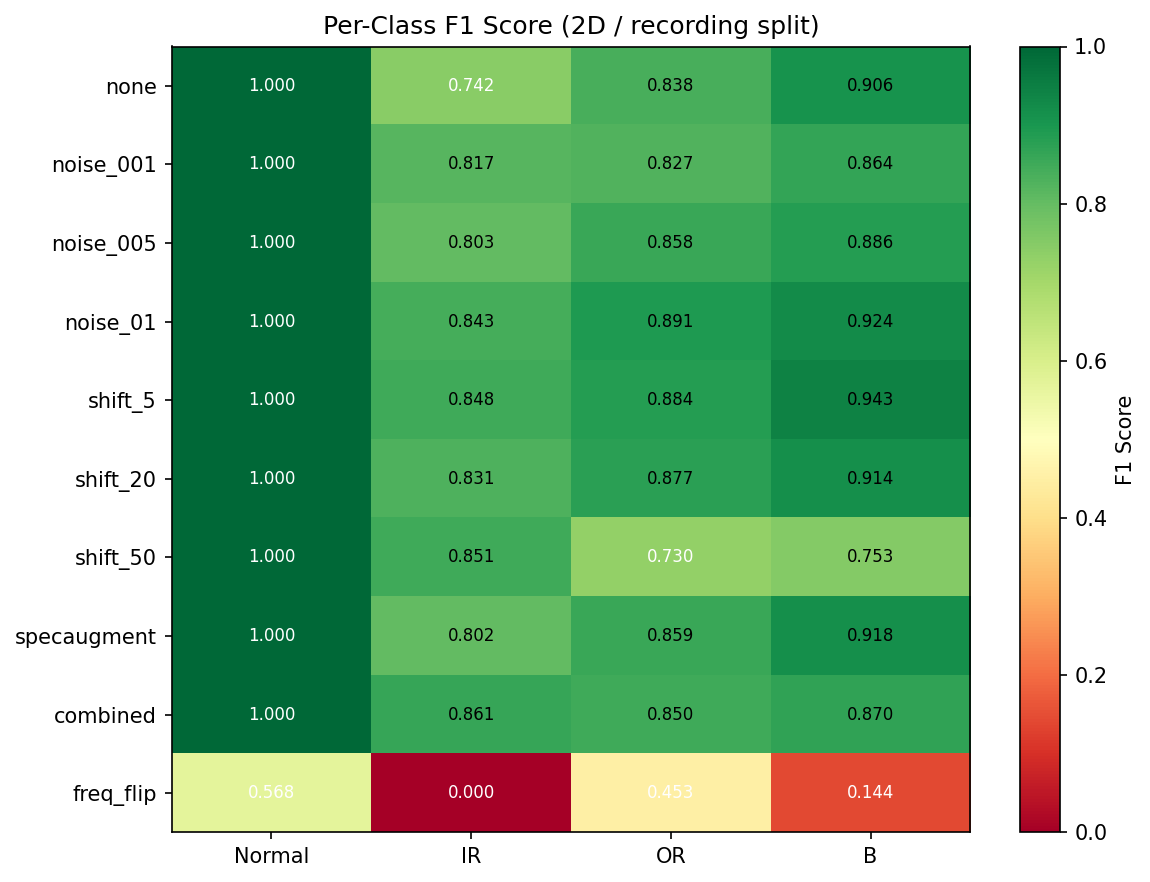
\includegraphics[width=0.48\textwidth]{../results/figures/per_class_2d_recording.png}
\caption{Per-class F1 heatmaps. Left: 1D-CNN. Right: 2D-CNN.}
\label{fig:pc}
\end{figure}

\begin{figure}[H]
\centering
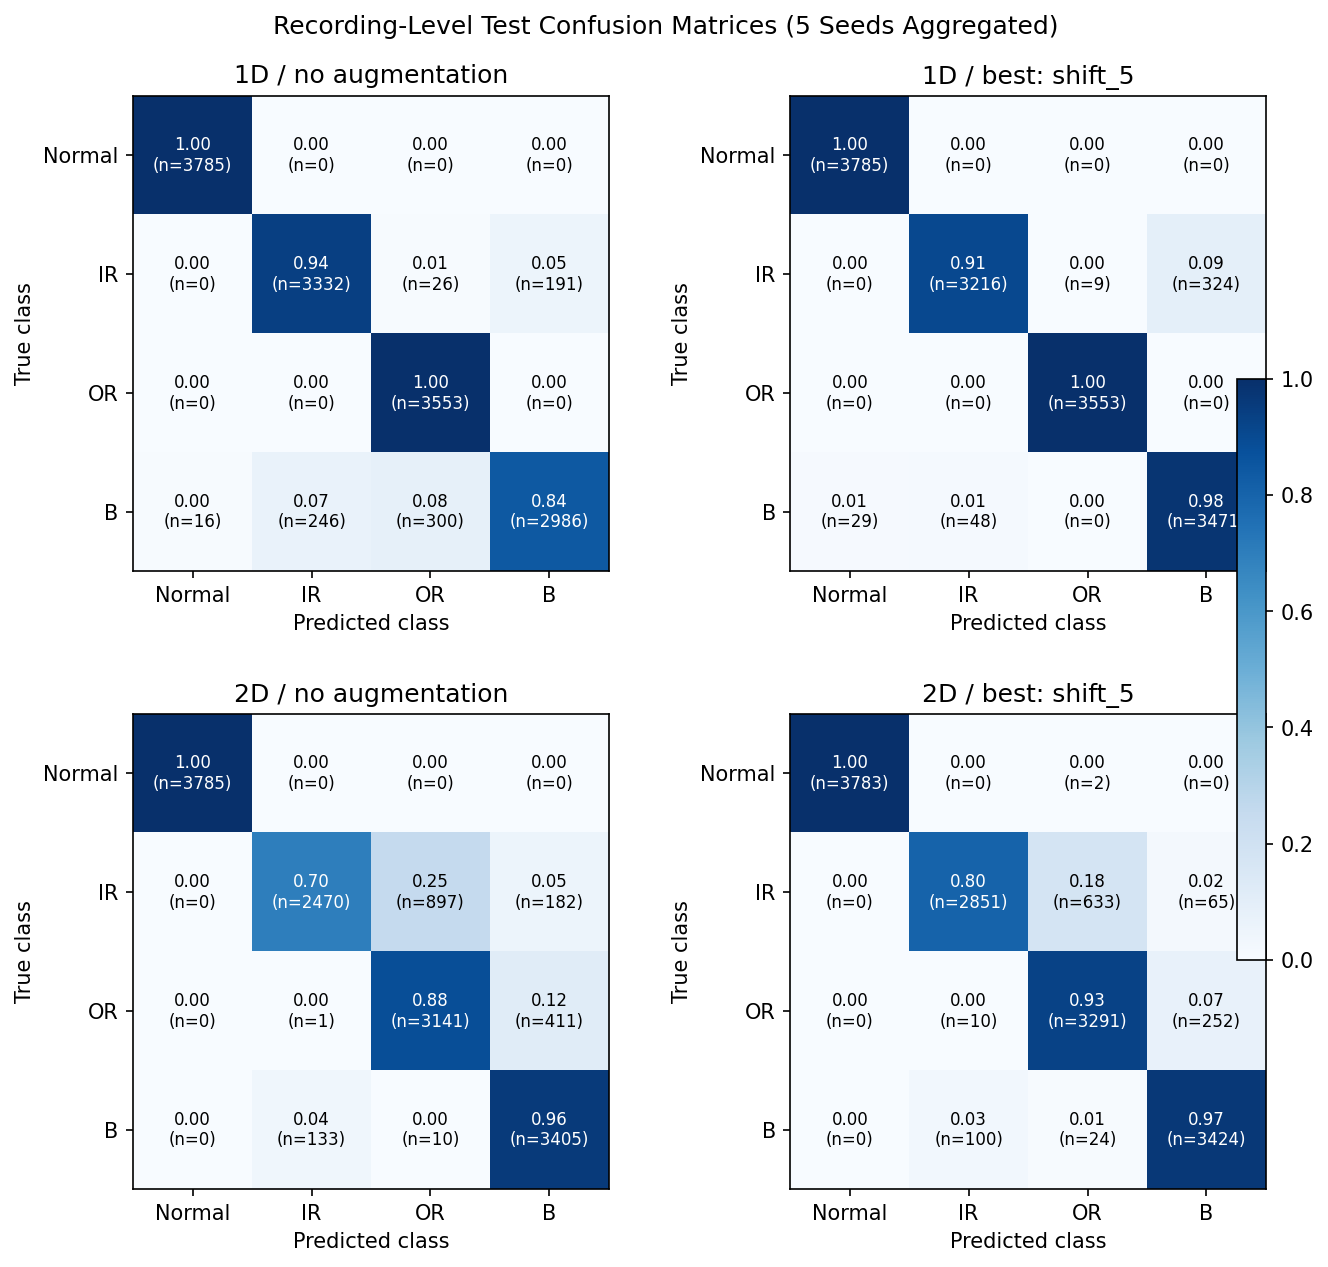
\includegraphics[width=\textwidth]{../results/figures/confusion_matrices_recording.png}
\caption{Row-normalized recording-level test confusion matrices aggregated across five seeds for selected baseline and augmentation conditions. Cell labels also report raw aggregated counts.}
\label{fig:confusion}
\end{figure}

\subsection{Gap-Recovery Analysis}

% [Gap-recovery解读]：Δrec是本文的核心指标，必须用一句话定义清楚。negative Δrec意味着增强后比不增强还差——这很反直觉，要引起审稿人注意。
Table~\ref{tab:gap} reports $\Delta_{\text{rec}}$---the proportion of the no-augmentation random-to-recording protocol gap recovered by each augmentation. The best values are 0.5255 (1D) and 0.3263 (2D), both from a 5-sample shift.

% AUTO-GENERATED by src/summarize_results.py; do not hand-edit.
\begin{table}[htbp]
\centering
\caption{Gap recovery relative to the no-augmentation random-to-recording protocol gap.}
\label{tab:gap}
\resizebox{\textwidth}{!}{%
\begin{tabular}{lrrrrrr}
\toprule
Augmentation & Gap (1D) & $\Delta_{\rm rec}$ (1D) & $d$ (1D) & Gap (2D) & $\Delta_{\rm rec}$ (2D) & $d$ (2D) \\
\midrule
None & 0.0569 & +0.0000 & 0.9262 & 0.1143 & +0.0000 & 1.4697 \\
Noise 0.01 & 0.0620 & -0.0879 & 1.7729 & 0.1190 & -0.0429 & 1.8234 \\
Noise 0.05 & 0.0371 & +0.3497 & 1.5421 & 0.1098 & +0.0385 & 1.9189 \\
Noise 0.10 & 0.0646 & -0.1371 & 0.9600 & 0.0809 & +0.2905 & 1.2869 \\
Shift 5 & 0.0271 & +0.5255 & 0.8412 & 0.0768 & +0.3263 & 1.4306 \\
Shift 20 & 0.0730 & -0.2847 & 1.2076 & 0.0906 & +0.2056 & 1.6770 \\
Shift 50 & 0.0603 & -0.0580 & 0.9596 & 0.1520 & -0.3316 & 1.0632 \\
Spectral/time mask & 0.0560 & +0.0176 & 0.8384 & 0.0986 & +0.1339 & 1.4576 \\
Combined & 0.0665 & -0.1670 & 1.1148 & 0.1037 & +0.0910 & 2.0354 \\
FFT magnitude reversal & 0.0043 & -9.4956 & 0.0567 & 0.0569 & -4.3193 & 0.6640 \\
\bottomrule
\end{tabular}
}
\end{table}


Figures~\ref{fig:gap1d}--\ref{fig:gap2d} visualize the gap-recovery landscape.

\begin{figure}[H]
\centering
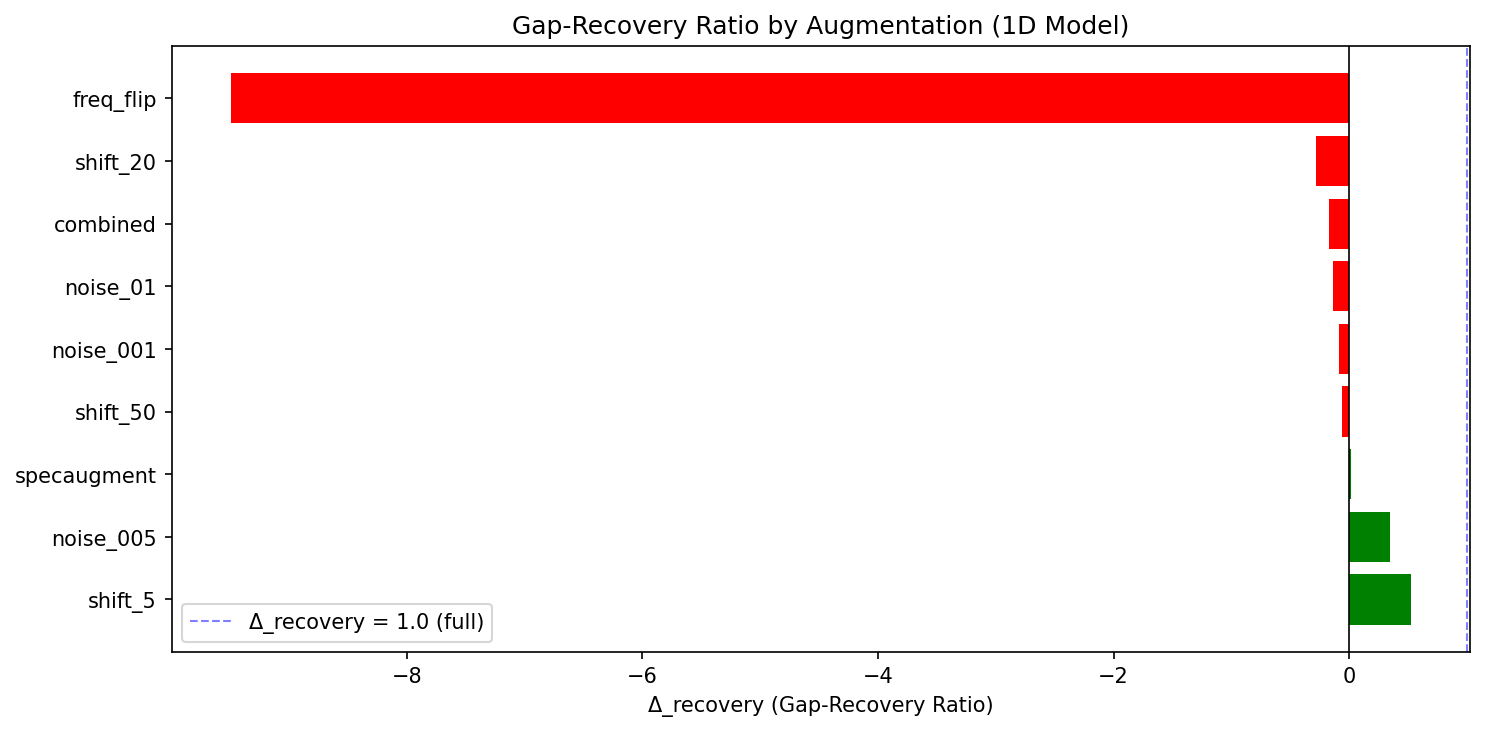
\includegraphics[width=\textwidth]{../results/figures/gap_recovery_1d.png}
\caption{Gap-recovery ratio by augmentation (1D-CNN).}
\label{fig:gap1d}
\end{figure}

\begin{figure}[H]
\centering
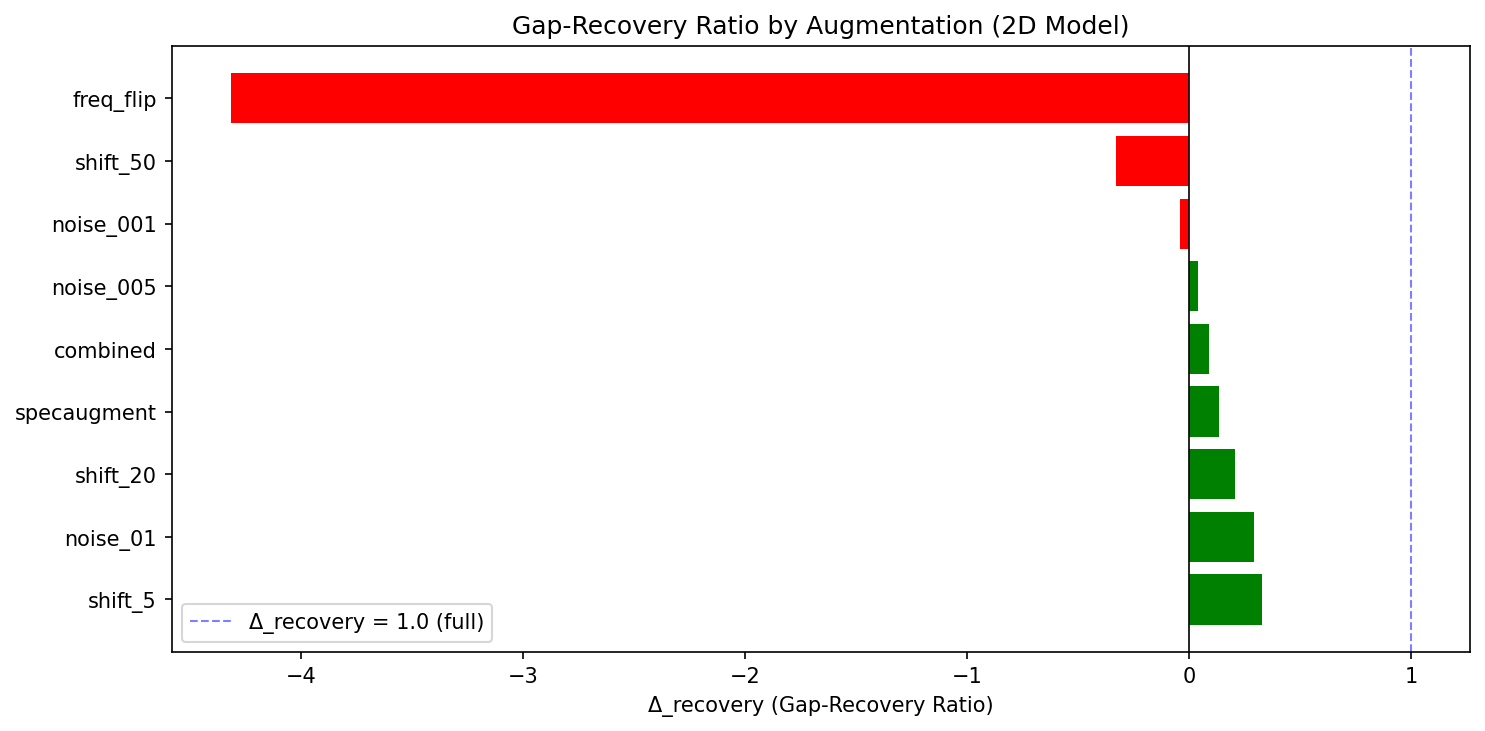
\includegraphics[width=\textwidth]{../results/figures/gap_recovery_2d.png}
\caption{Gap-recovery ratio by augmentation (2D-CNN).}
\label{fig:gap2d}
\end{figure}

\subsection{Grouping-Variable Ablation}

% [分组解读]：fault-size 准确率最低，但覆盖不匹配，不能转化为因果重要性排序。
Table~\ref{tab:ablation} compares no-augmentation accuracy across the three grouping stress tests. Fault-size grouping is lowest (0.6508 for 1D and 0.4920 for 2D), compared with recording grouping (0.9429 and 0.8856) and load grouping (0.9607 and 0.9779).

% AUTO-GENERATED by src/summarize_results.py; do not hand-edit.
\begin{table}[htbp]
\centering
\caption{Descriptive grouping stress-test accuracy (mean $\pm$ std across 5 seeds). Load and fault-size strategies use unequal group counts and are not causally comparable.}
\label{tab:ablation}
\begin{tabular}{lccc}
\toprule
Model & By Load (2/1/1) & By Recording & By Fault Size (1/1/1) \\
\midrule
CNN--1D & 0.9607 $\pm$ 0.0331 & 0.9429 $\pm$ 0.0777 & 0.6508 $\pm$ 0.1131 \\
CNN--2D & 0.9779 $\pm$ 0.0286 & 0.8856 $\pm$ 0.0984 & 0.4920 $\pm$ 0.1182 \\
\bottomrule
\end{tabular}
\end{table}


This ordering is descriptive, not causal. Recording, load, and fault-size strategies contain 23/7/10, 20/10/10, and 14/13/13 train/validation/test recordings, respectively; load also uses 2/1/1 groups, whereas fault size uses 1/1/1. Lower fault-size accuracy is therefore consistent with a difficult stress test but is confounded by reduced training coverage.

% ================================================================
\section{Efficiency / Robustness / Physical Consistency}
% ================================================================

% [H3未获支持]：报告逐模型主分析、排除负对照的敏感性分析，以及样本量和池化独立性限制。
H3 is not supported. Across all nine augmentations, the per-model Spearman correlations between symmetric envelope-spectrum fault-band fidelity and gap recovery are positive but non-significant: $\rho=0.4333$, $p=0.2440$ for 1D and $\rho=0.3167$, $p=0.4064$ for 2D (Figure~\ref{fig:h3}). Because the negative control has extreme recovery values, we repeat the analysis without it; correlations fall to $\rho=0.1905$ ($p=0.6514$) and $\rho=0.0238$ ($p=0.9554$). An exploratory pooled value is not used inferentially because both models reuse the same nine fidelity measurements.

\begin{figure}[H]
\centering
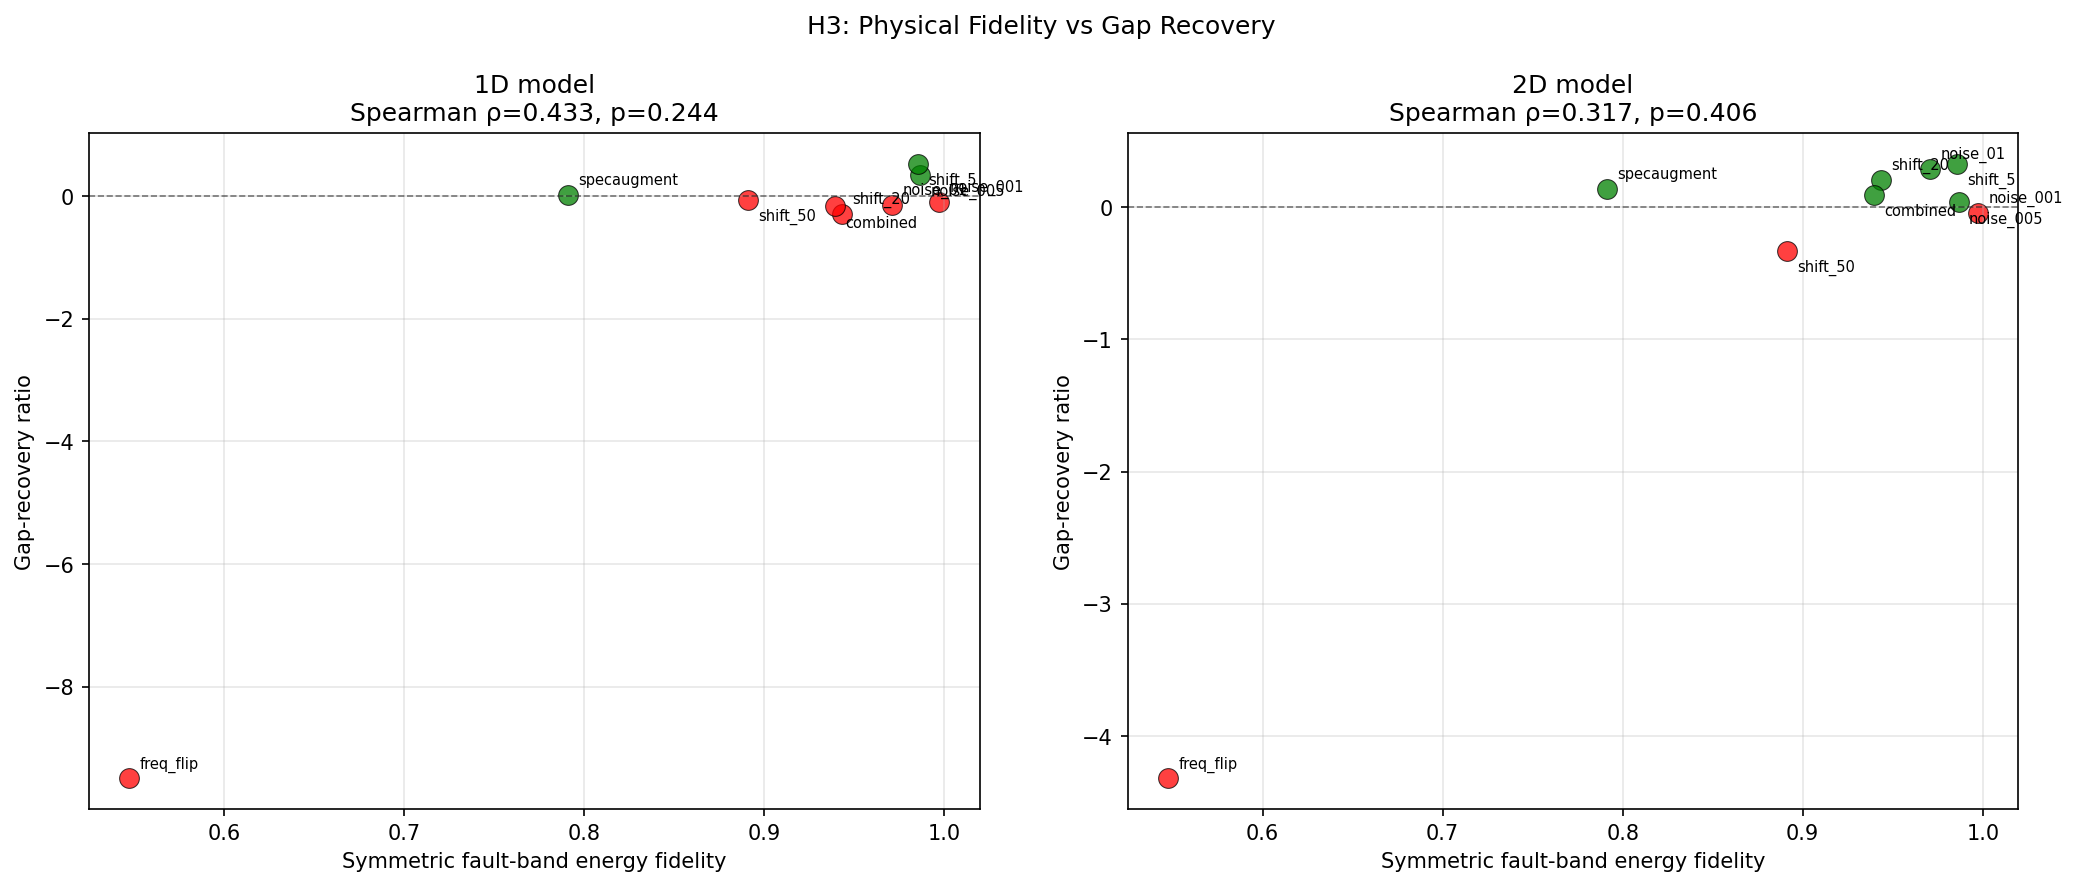
\includegraphics[width=\textwidth]{../results/figures/h3_physical_fidelity_correlation.png}
\caption{H3: Symmetric physical energy fidelity ($F_{\text{energy}}$) vs.\ gap recovery ($\Delta_{\text{rec}}$), reported separately by model.}
\label{fig:h3}
\end{figure}

\textbf{Exploratory contamination check.} A paired, single-seed auxiliary test evaluates selected recording-level models on common clean and noise-contaminated test realizations up to $\sigma=0.10$. It shows little degradation over the tested range, but one seed cannot establish statistical robustness or rank augmentation strategies. The complete values are retained in \texttt{results/tables/contamination\_robustness.json} and are not used to support H1--H3.

% ================================================================
\section{Ablation}
% ================================================================

\subsection{Single vs.\ Combined Augmentation}

% [单增强vs组合增强]：测试的组合条件不及 shift 5，但不外推为所有 stacking 均有害。
Combined augmentation does not outperform the best single augmentation. Under recording-level splitting, combined reaches 0.9334 for 1D and 0.8960 for 2D, whereas the 5-sample shift reaches 0.9728 and 0.9229. This result does not show that stacking is generally harmful, but it provides no benefit for the tested noise-plus-shift combination.

\subsection{Grouping Stress-Test Comparison}

% [分组压力测试小结]：重申精确覆盖差异与描述性边界。
The fault-size strategy has the lowest observed accuracy (0.6508/0.4920), but it also trains on one of three diameter groups and only 14 recordings. Table~\ref{tab:ablation} therefore identifies a demanding configuration rather than causal variable importance.

% ================================================================
\section{Discussion}
% ================================================================

% [H1讨论]：先确认成立再指出局限。2D弱于1D的现象可以引发关于spectrogram信息损失的讨论。
\textbf{H1 (partial recovery)} is supported. The best tested augmentation, a 5-sample shift, recovers 52.55\% of the 1D protocol gap and 32.63\% of the 2D gap; neither closes the gap.

% [H2讨论]：用Cohen's d的定量语言确保论点的统计严谨性。proper evaluation protocol一词强调方法论意义。
\textbf{H2 (protocol-gap dominance)} is supported operationally: the largest recovery ratio remains below one for both models. This experiment cannot assign a causal fraction of the gap to exact shared-sample leakage versus the broader unseen-recording distribution shift.

% [H3讨论]：不显著结果只能表述为“未获支持”，不能证明保真度无关或确定替代机制。
\textbf{H3 (physical fidelity)} is not supported. Neither per-model test is significant, with or without the negative control. This null result does not establish that physical fidelity is irrelevant; nine augmentation-level observations provide limited power and the metric captures only envelope-spectrum band energy.

% [种子敏感性]：报告前三个与全部五个配置种子的差异，不宣称五个种子普遍充分。
\textbf{Seed-count sensitivity.} Using only the first three configured seeds would give recording baselines of 0.9961 (1D) and 0.9631 (2D). Including seeds four and five changes the five-seed means to 0.9429 and 0.8856, shifts of 5.32 and 7.75 percentage points. Five seeds still do not guarantee stable population estimates, but the observed change shows that three were inadequate here.

% [故障尺寸压力测试]：低准确率值得后续匹配覆盖实验，但当前不能分离尺寸偏移和训练覆盖效应。
\textbf{Fault-size stress test.} Its low 0.6508/0.4920 accuracy warrants follow-up with a matched-coverage design. The present comparison cannot separate fault-size shift from the fact that this strategy trains on fewer recordings and only one diameter group.

% ================================================================
\section{Limitations}
% ================================================================

% [局限性列表]：覆盖手册要求的基准外推、人工故障、随机窗口泄漏、条件依赖、AI审计等边界。
\begin{enumerate}[nosep]
    \item \textbf{Single benchmark and artificial faults}: All experiments use CWRU's seeded laboratory faults. High accuracy here does not establish field readiness or performance on naturally evolving damage.
    \item \textbf{Condition dependence}: Only the drive-end 12\,kHz accelerometer is used. Results may change with load, speed, sensor location, sampling rate, or segmentation; fan-end 48\,kHz data would provide one sensitivity check.
    \item \textbf{Leakage-prone comparator}: Random adjacent-window splitting intentionally permits source recordings and shared samples to cross partitions. Its result is a diagnostic comparator, not an estimate of unseen-recording performance.
    \item \textbf{Fixed augmentation parameters}: Parameters chosen a priori; sensitivity not explored.
    \item \textbf{Offline augmentation}: Each transform is sampled once per run and replaces, rather than expands, the training partition; online per-epoch resampling may behave differently.
    \item \textbf{CNN architectures only}: Results may differ for Transformer or MLP architectures.
    \item \textbf{50-epoch ceiling}: Eight of 200 runs reach their best validation accuracy in epochs 45--50; this best-epoch diagnostic does not prove formal convergence.
    \item \textbf{Physical metric and sample size}: Symmetric band-energy fidelity covers one physical dimension, and H3 has only nine augmentation-level observations per model.
    \item \textbf{Grouping comparability}: Group counts and training-recording counts differ, so grouping accuracy cannot be interpreted as causal variable importance.
    \item \textbf{Reduced robustness scope}: The planned all-pairs cross-load experiment was not completed, and the contamination check uses one seed. Neither supports a general robustness claim.
    \item \textbf{AI-assisted workflow}: AI assisted coding, analysis, drafting, and review. Artifact-level verification reduces but cannot eliminate transcription, framing, or citation-audit error; responsibility for the claims remains with the authors.
\end{enumerate}

% ================================================================
\section{Conclusion}
% ================================================================

% [结论段]：遵循标准结构——重申核心发现→量化效果→指出最限制因素（跨严重度泛化）→方法论建议→开放数据承诺。不需要新信息，只需要强有力地复述Results+Discussion。
Matched-preprocessing evaluation on CWRU yields no-augmentation random-to-recording protocol gaps of 0.0569 (1D) and 0.1143 (2D). A 5-sample shift recovers 52.55\% and 32.63\%, while the destructive negative control collapses performance. H3 is not supported in either model or in the sensitivity analysis without the control. Fault-size grouping is the hardest observed stress test, but unequal coverage prevents a causal ranking. The seed diagnostic, exact split assignments, complete logs, matrices, and generated tables make the limits as well as the findings independently checkable.

% ================================================================
\section{Reproducibility Statement}
% ================================================================

% [可复现性声明]：包含代码位置、种子列表、日志位置、再生指令四要素。凡是无法仅凭论文正文复现的信息，都应在此披露。
All code, selected-file hashes, exact split manifests, experimental configurations, and results are included in the project repository. Random seeds (42, 123, 456, 789, 1024) are fixed across all experiments. The exact A10 package versions are recorded in the repository's \texttt{environment} directory, in \texttt{requirements-a10-lock.txt}. Set \texttt{CWRU\_DATA\_ROOT} to the directory containing the selected source files and, for GPU execution, set \texttt{CWRU\_DEVICE=cuda}. Run:
\begin{quote}
\small
\texttt{python src/run\_all.py}\\
\texttt{python src/verify\_release.py}
\end{quote}
The first command regenerates the evidence, while the second checks run counts, configurations, matrices, manifests, generated tables, figures, and PDF freshness. Per-epoch logs for all 200 main runs are included. Raw CWRU files are not redistributed.

% ================================================================
\section{AI-Use Disclosure}
% ================================================================

% [AI使用披露]：按功能分类——代码实现、调试、起草。结尾的universal denial是防止M3（幻觉结果）的基础防护。
The work used DeepSeek via OpenCode CLI for initial pair-programming, debugging, analysis, and drafting. OpenAI Codex subsequently performed an independent course-compliance and data-copy audit, identified protocol/evidence mismatches, implemented the documented repairs, orchestrated an isolated A10 rerun, and reconciled the release artifacts. The complete interaction summary and verification trail are recorded in \texttt{prompts/prompt\_log.md}. Numerical statements were checked against generated JSON/CSV artifacts, dataset statements against the material passport and manifests, and citations against the retained bibliography/source records. Numerical results and figures come from code executed on the selected CWRU files; AI did not invent missing results. The authors retain responsibility for the final interpretation and disclosure.

% ================================================================
% REFERENCES
% ================================================================
\begingroup
\small
\bibliographystyle{ieeetr}
\bibliography{refs}
\endgroup

\end{document}
